\documentclass[12pt]{article}
\usepackage[utf8]{inputenc}
\usepackage[LGR, T1]{fontenc}
\usepackage[greek.ancient,english]{babel}
\usepackage{alphabeta}
\usepackage{tipa}

\usepackage[letterpaper, margin = 1in]{geometry}
\usepackage{fancyhdr}
\usepackage{titling}
\usepackage{titlesec}
\usepackage{hyperref}
\usepackage{lastpage}
%\usepackage{lipsum}
\usepackage{amssymb}
\usepackage{setspace}
\usepackage{stmaryrd}
\usepackage{rotating}

\usepackage{hanging}
\usepackage{tabularx}
\usepackage{multirow}
\usepackage{array}
\usepackage{multirow}
\renewcommand\tabularxcolumn[1]{m{#1}}
\usepackage{arydshln}

\usepackage{tikz}
\usepackage{tikz-qtree}
\usepgflibrary{arrows}
\usetikzlibrary{positioning,shapes.multipart}
\usetikzlibrary{tikzmark}
\usetikzlibrary{fit}
%\usepackage{tree-dvips}

\usepackage{linguex}

\usepackage[backend=biber, style=apa]{biblatex}
\setlength{\bibhang}{0.5in}
\addbibresource{weaving.bib}
\usepackage{csquotes}
\DeclareLanguageMapping{english}{english-apa}

%\usepackage{gb4e}

\usepackage{graphicx}
\graphicspath{ {./images/} }

\title{Discrete Infinity and Ring Structure in Penelope's Weaving Trick}
\author{Ian Thomas White}
\date{}

\makeatletter
\renewcommand{\maketitle}
{
\begin{flushleft}
\textbf{{\large\@title}}
\newline
\@author
\end{flushleft}
}
\makeatother

\titleformat*{\section}{\large\bfseries}
\titleformat*{\subsection}{\medium\bfseries}
\titleformat*{\subsubsection}{\small\bfseries}

\pagestyle{fancy}
\fancyhf{}
\lhead{Ian Thomas White}
\chead{Weaving}
\rhead{\thepage \ of \pageref{LastPage}}

% \linespread{1.6}
\doublespacing
\widowpenalty=100000
\clubpenalty=100000


\begin{document}

\thispagestyle{empty}

\begin{singlespacing}
\maketitle
\tableofcontents
\end{singlespacing}

\newpage

\section{Introduction}\label{intro}

Weaving and related textile activities are among the most widespread and long-lasting literary motifs across the world, and the so-called Western canon is no exception.\footnote{ See, e.g., Kruger 2001 for some cross-cultural comparisons.} The weaving motif has a longstanding history in both literature and literary studies, being well-attested since at least Homer.\footnote{ For the ancient world, it will suffice to merely mention the weavings of Penelope, Helen, Philomela, and Arachne, as well as \textit{peplos}-bearing Athena's divine purview over weaving. See Fanfani, Harlow, \& Nosch 2016, and its containing book more generally, for extended use of the motif in ancient literature and theory.} Hence, too, the myriad, long-lived metaphors in modern English: ``to thread the plot'', ``to tell a yarn'', ``to lose the thread'', ``to weave a tale'', etc.\footnote{ See also Guilleux (2016) for many cross-linguistic reflexes of the weaving metaphors.}

The prevalence of the weaving motif, accordingly, has not been lost on modern commentators on ancient works. The motif has also proven to be a fruitful field for research, especially as scholarship has increasingly discovered the mechanical techniques that ancient weavers would have used.\footnote{ Most notably since Barber 1991.} As it stands, classics scholarship on weaving can be fairly siphoned into three general camps: a) research focused on the linguistic, usually etymological, meanings of weaving terms, whether in literary contexts or not;\footnote{ See, most prominently, Schmitt 1967 and Durante 1960.} b) research focused on the literal mechanical techniques of ancient weaving\footnote{ Again, see Barber 1991, among others listed below.}; c) research focused on deriving broader, often meta-poetic, implications from the weaving motif as it's deployed in ancient literature.\footnote{ There are numerous examples in this camp, some of which are discussed below. The higher-order implications generally fall under some subset of poetic/literary theory, (ancient) gender theory/dynamics, and/or political dynamics.} 

The first two camps, (a) and (b), can be grouped, descriptively, as ``technical'', while the third is ``higher-order''. Less common than any individual type, though not non-existent, are works that try to combine the above types (a) and/or (b) with (c).\footnote{ See Nagy 2010ab for examples of (a)+(c) and Harlizius-Kl\"{u}ck \& Fanfani 2016 for (b)+(c).} To my ear, those works that have attempted to merge technical linguistic or mechanical discoveries to larger literary questions have provided only tenuous links between the two groups. Neither etymology nor mechanics have any \textit{a priori} or direct mapping onto higher-order literary questions.\footnote{ Again, Nagy 2010ab and Harlizius-Kl\"{u}ck \& Fanfani 2016 are examples of this pitfall. Still, I don't mean to say that the higher-order questions can only be reasonably discussed pending some reasonable discussion of etymology or mechanics, only that, should both modes be discussed, the mapping must be made explicit.} Rather, if (i) certain linguistic elements in some literary object refer to particular outside (weaving) mechanics, and (ii) it's assumed that the literary object is privy to such mechanics and that it seeks to treat them in a robust and relatively precise way,\footnote{ Of course, the object can be so privy even if the author/s is/are not. This is not a trivial assumption, but it is one that literary studies in general depends upon, namely that literary deployments are actively operant in some analyzable way.} then (iii) an analysis must explicitly show how that literary object produces or discusses such a treatment. That is to say, the outside (weaving) mechanics must be explicitly mapped to the literary deployment of the linguistic elements, not only to the linguistic elements themselves. The mapping to only linguistic elements is, as far as literary questions are concerned, simply tautological, since the mechanics-linguistic mapping is assumed to obtain in the first place for any subsequent literary analysis to occur.

By analyzing Penelope's famous weaving trick in Homer's \textit{Odyssey}, the present paper seeks to uncover one potential mapping from weaving mechanics to literary questions. As my theoretical starting point, I assume that the ancient Greek poetic form called a \textit{humnos} had a particular, well-defined structure, as developed by Nagy (2010ab), and that the Homeric epics, among other related texts, are well-versed in and utilize this structure. Oversimplifying for now, the word \textit{humnos} itself and its structure are based on weaving and consist of particular, requisite beginnings, middles, and ends. Furthermore, literal weaving mechanics of the time had particular, requisite attributes, notably described by Harlizius-Kl\"{u}ck \& Fanfani (2016). For present purposes, it suffices to say that a web had a requisite beginning that, crucially, determined the dimensions of the web before it was fully woven. The beginning of a \textit{humnos}, furthermore, is itself based on a weaving metaphor, though not directly that of the beginning of a literal web.

Since the \textit{humnos} structure and etymology operate over weaving metaphors, there must be some implicit literary mapping between weaving mechanics and the \textit{humnos} structure, but, again, this mapping is by no means apparent, neither in the mechanics nor in the terms' definitions. I will show that, in fact, a very difficult problem obtains when the weaving-\textit{humnos} mapping is attempted. Namely, unlike weaving, the \textit{humnos} has no \textit{a priori} way of ending itself, no beginning that entails an end at some pre-defined point. Still, it turns out that literal weaving and the \textit{humnos} can both be modelled as explicit structures (here, as ``equations''), allowing explicit mapping between them. By breaking the bounds of such structures, the \textit{humnos} risks never ending and thereby producing a discrete infinity. The problem of discrete infinity is thus \textit{a priori} the case in my reconstruction of Nagy's \textit{humnos}, but the same problem obtains \textit{a posteriori} in the \textit{Odyssey}. Using Penelope's trick I show that the \textit{Odyssey} is quite aware of the problem of discrete infinity, such that Penelope's web and, by extension, the \textit{humnos} in general, would iterate itself indefinitely and would never be able to end without some outside force.\footnote{ Hence, many prior treatments of Penelope's web, without invoking explicit weaving mechanics, notice that the meta-poetic import potentially implies some sort of unending poetics, despite the fact that the web ends.} Finally, just as the \textit{Odyssey} is aware of this problem, I show, too, that the epic provides a solution to it, though one that's distinct from literal weaving. The epic uses the well-cited and discussed literary ring-structure as a way to proscribe the problem of discrete infinity. Namely, the \textit{Odyssey} ties Penelope's trick to a ring-structure that operates across the entire epic, ultimately entailing a particular end to the otherwise unending trick.

Thus, this paper attempts to fill a very particular gap in recent scholarship by showing how discoveries in ancient weaving mechanics can be explicitly mapped to literary devices. Herein, Section 2 summarizes important, relevant linguistic weaving metaphors in Greek literature, as well as our current understanding of the literal weaving mechanics therein. Section 3 summarizes and develops the \textit{humnos} structure in the works of Nagy, ultimately deriving a more coherent and explicit structure for the form. I provide a formula for the \textit{humnos} structure that shows how it relates in explicit terms to the process of weaving, as well as how the \textit{humnos} and literal weaving seem to diverge in \textit{a priori} terms. Section 4 provides my analysis of Penelope's trick, showing that the \textit{Odyssey} displays and seeks to remedy the same, potential discrete infinity of poetry modelled on weaving. The remedy therein, I claim, is the ring structure. Finally, Section 5 offers some larger theoretical implications of the foregoing discussion.

\section{Weaving Background}\label{background0}

In this section I offer a brief summary of relatively modern work on the subject of weaving in comparative linguistics and in textile studies. I do so without any pretense of providing a comprehensive run-through of the literature on weaving; instead, I highlight and detail the most relevant information to the project at hand.

\subsection{Linguistic Work}\label{background1}

Extensive linguistic work has shown the ingrained and persistent use of a variety of textile metaphors (usually qua vehicle) across Indo-European languages up to the present day, Greek being no exception.\footnote{ Much of the following framework and data comes from Guilleux 2016. See the bibliography there for a number of important works. See Schmitt 1967 and Durante 1960 for more in-depth studies.} I wish here to highlight well-established textile metaphors that are relevant for Greek literature and for the discussion to follow.\footnote{ These metaphors seem to occur in reconstructed Indo-European through at least Classical Greek literature, though with different emphases, frequencies, and casts. See the above cited literature.}

\noindent \hfill \par
\noindent \textbf{Thread as Fate/Life} \\
The \textit{moirae}/fates and, by extension, fate itself are traditionally related to the spinning of fabric, a step that produces thread before weaving takes place. This is most evident in the name (at least since Hesiod) of one of the fates, Κλωθώ (`spinner'). The other two names, Λάχεσις `apportioner') and Ἄτροπος (`unturned'), can be somewhat easily given textile-related interpretations: the former measures the thread and the latter cuts it.\footnote{ See Bergren 2008: 32 for the translations of these names. Λάχεσις derives from λαγχάνω `to obtain by lot' (Beekes 2009).} Moreover, Λάχεσις, Κλωθώ, Ἄτροπος are commonly each linked to the past, present, future, respectively.\footnote{ See Giannakis 1988 and Alfaro 2016 citing Plato \textit{Rep.} 616b-c9.} Important verbs are κλώθω and νήθω, which both mean `to spin', including, e.g., collocations such as κλώθω τέλος βίου (`I spin the end of life').\footnote{ Guilleux 2016 citing Quintus Smirnaeus 11.141}

\noindent \hfill \par
\noindent \textbf{Un/winding a spool as life events} \\
Greek features the verb (ἐκ)τολυπεύειν, which comes from the noun τολύπη. The noun means most literally `a clew of wool or yarn'. The verbs thereby mean `to wind wool or yarn into (out of) a clew' but also have the extended meaning of `(making someone) undergo difficult labors'.\footnote{ Beekes 2009 and Guilleux 2016.} This metaphor thereby has a negative valence, being usually associated with difficulty or pain.

\noindent \hfill \par
\noindent \textbf{Weaving as Speech/Poetry} \\
This metaphor relates the act or product of some type of poetic utterance to the act or product of weaving, and it is the most discussed and the most debated metaphor in the given textile metaphor domain.\footnote{ Edmunds (2012) emphasizes that ``a loom is essentially more a method than a thing'', citing Penelope's web, to be discussed further below.} The verb for `to weave', including a whole host of varying abstract extensions, is ὑφαίνω. There is debate as to whether ὕμνος (`song, hymn') is etymologically related to ὑφαίνω, but many seem to assume that it is.\footnote{ Beekes (2009) says this derivation is ``phonetically difficult''. See Nagy 2010a: 229-230 and Harlizius-Kl\"{u}ck \& Fanfani 2016: 89 for more sanguine outlooks on the derivation.} In any case, the explicit association between ὔμνος and ὐφαίνω in Greek literature is well-established at least since Pindar, but it is somewhat disputed for Homer. Nagy (1996b) refutes well Scheid and Svenbro's (1996) claims that the weaving-poetry metaphor doesn't exist in Homer. According to Nagy, such a metaphor exists as an operative remnant in Homeric poetry, though explicit formulations are indeed somewhat rare.\footnote{Again, see Nagy 2010a. Snyder (1981: 194) treads a middle ground, saying that ``while Homer himself never actually describes poetic activity as analogous to weaving at the loom, his frequent references to metaphorical and literal weaving, as well as his juxtaposition of actual weaving and singing, lay the foundation for the lyric poets' descriptions of their own webs''. See also Nagy 2010b. Guilleux (2016: 12) says ``it is quite rare in ancient Greek''.} The most conspicuous and oft-noted collocation is μύθους καὶ μήδεα ὕφαινον (`they wove words and schemes', \textit{Iliad} iii.212),\footnote{ For Nagy (1996a), μύθος is marked, poetic speech, relative to the generic ἔπος. See also Martin 1989.} and Helen's battle-scene weaving (Iliad iii.125-128) is usually considered in this light. Nagy (2010b) also claims that ποικίλος (`varied') and ποικίλλειν (`to make varicolored') is constitutive of Homeric verse and modelled after Athena's Panathanaeic \textit{peplos}.\footnote{ Wace 1948 condemns the common translation of these terms as `embroidery'.} The verb πλέκειν (`plait') and its derivatives can similarly be used with words for speech. It's also worth noting that another word for `to weave' is κρέκειν (literally, `to strike with a \textit{kerkis}'), which can also be used for `to play an instrument', and a number of literal and metaphorical similarities obtain between weaving and music.\footnote{ This is not directly attested in Homer, however. See Snyder 1981 and Nosch 2014.} Finally, προοίμιον (`opening, introduction'), based on the root \textit{-oim-} (`thread'), is often interpreted as the `(starting) thread' of a song when in a poetic context.\footnote{ See Nagy (1996b, 2010a), who then conflates `threading' with `stitching', and Harlizius-Kl\"{u}ck \& Fanfani (2016). Beekes (2009) is skeptical on this point.} This makes \textit{-oim-} (`thread') based metaphors a particular subcase of weaving more general.

\noindent \hfill \par
\noindent \textbf{Sewing/Stitching as Poetry} \\
Sewing and weaving as vehicles for poetry are often conflated, but it's worth distinguishing them.\footnote{ Guilleux (2016) doesn't reference the distinction. Nagy (1996b) essentially makes sewing a special form of weaving.} The important verb here is ῥάπτειν (`to stitch (together)'), which is notably collocated with ἀοιδή (`song') to form ῥαψῳδός (`song-stitcher').\footnote{ Nagy 1996b.} Nagy (1996b, 2010a) claims that `stitching', like varicolored weaving,\footnote{ I will discuss how these two metaphors interact below.} is constitutive of Homeric verse and even derives `Homer' from the root \textit{-ar-}, e.g., ἀραρίσκειν (`to join together'), such that the name signifies `he who joins together'.\footnote{ This is funded primarily through a carpentry metaphor, which extends into a weaving metaphor (Nagy 1996b: 74-75).} Finally, ὕμνος can be derived from a root meaning `to sew, stitch' instead of the above weaving-based derivation.\footnote{ Beekes 2009.} Apart from possibly ὕμνος, the stitching metaphor is not traced to Indo-European, unlike the weaving metaphors. Furthermore, stitching doesn't seem to refer to something like modern sewing, in which a separate thread connects two or more cloths; instead, it refers to a range of actions that use threads from one cloth to connect to itself another cloth.\footnote{ Harlizius-Kl\"{u}ck \& Fanfani 2017. See the discussion below.}

\noindent \hfill \par
\noindent \textbf{Weaving as Cunning/Trickery} \\
Acts of cunning and trickery (δόλος, μῆδος, κέρδος) are not uncommonly described using weaving terms, or at least with indirect reference to weaving. Penelope's web, to be discussed in detail below, is a common example of this metaphor.\footnote{ Though Guilleux (2016) wrongly categorizes δόλους...τολυπεύω (\textit{Oddyssey} xix.137) as weaving instead of winding.} Similarly, Odysseus says δόλους καὶ μῆτιν ὕφαινον (`I was weaving tricks and craft'). The verb πλέκειν (`to plait') and ῥάπτειν (`to stitch, sew') and their derivatives can also be used with words for cunning and trickery.\footnote{ See also Detienne and Vernant 1974.}

\noindent \hfill \par
\noindent \textbf{Weaving as City} \\
Scheid and Svenbro (1996) detail a metaphor in which the city is likened to a woven cloth. Supposedly, this metaphor was ``a linguistic fact that was likely to underlie the idea of political weaving for all Greek speakers'', but most of the explicit examples come from post-Homeric sources, including Plato and Aristophanes. There may be some distant, underlying links to Homeric texts, e.g., in the Trojan offering of a peplos to Athena (\textit{Il.} VI:269-85). In any case, the ideal city is envisaged as an object made by harmonizing otherwise conflicting forces, like the warp and woof of a web. Other parts of (the craft of) wool-working (ταλασιουργική, explicit in Plato \textit{Pol.}, at least), e.g., carding (ξαίνειν) and spinning ((ἐκ)τολυπεύειν), are often included in this metaphor in varying ways. While this metaphor is important, I don't invoke it for the discussion of Penelope's web.

\subsection{Textile Work}

In relatively recent years, classical and archaeological research has uncovered much of the literal mechanics of a variety of ancient weaving machines and techniques.\footnote{ The urtext here is Barber 1991, but, unfortunately, I was unable to gain access to this book. The results therein that are relevant to the current paper, though, are summarized well enough in a number of places.} As above, I will summarize here the results relevant to the current paper.\footnote{ See Edmunds 2012 and  Harlizius-Kl\"{u}ck \& Fanfani 2016 for much of the data in this section.}

Greek weavers, in both Homeric and Classical ages, would have used a warp-weighted loom. In fact, this technique is dated to the early Neolithic period, which accords well with the archaic origin of weaving metaphors in Indo-European generally. The loom itself (ἱστός) sits upright (as suggested by ἱστός) on two vertical beams. The distinctive feature, as the name suggests, is that weights are tied to the vertical warp (ἱστός, στήμων, ἤτριον) threads in order to make them tense. Sets of warp threads are then arranged before or behind a variable set of horizontal beams, and in variable intervals, depending on the intended design. Requisite is the horizontal beam at the bottom of the loom (καῖρος) and at least one other horizontal beam, a heddle, toward the middle (κανών).\footnote{ The exact mechanics of heddle rods for Greek looms is disputed. See Edmunds 2012.} (In this case, the threads behind the lower rod are attached to the middle rod.) The loom is leaned against a wall to form a space, the shed, between the threads before and behind the bottom rod, and the heddle rod(s) can be moved toward and away from the weaver to create a counter-shed (i.e., to adjust which warp threads are in front and which behind each other.) The horizontal weft (κρόκη) threads are passed on a shuttle/spool/bobbin (πηνίον) one way through the shed between warp threads and then back the other way through the counter-shed (this activity being called βουστροφηδόν, `turning left and right (like an ox)').\footnote{ Nosch 2014.} Finally, the weft is beat into place using the κερκίς, which, according to Edmunds (2012), should be translated as `pin beater' and not `shuttle' or `spindle' as is common. Moreover, this item is the unique and distinguishing tool of the weaver.

The image below is a reconstruction of a web on the Chiusi skyphos from Harlizius-Kl\"{u}ck \& Fanfani (2016: 70, fig. 5.2). In it you can see the heading band attached to the top, and from it descend the web's warp threads, with weights at the bottom. The warp threads are alternately before and behind the horizontal rod at the bottom, and some of the warp threads are attached to the middle (heddle) rods, which can be moved forward and backwards (i.e., towards and away from the weaver/viewer) to create spaces (shed and counter-shed) between varying warp threads. The shuttle with the weft threads would be moved through those spaces. 
\noindent \hfill \par

\begin{center}
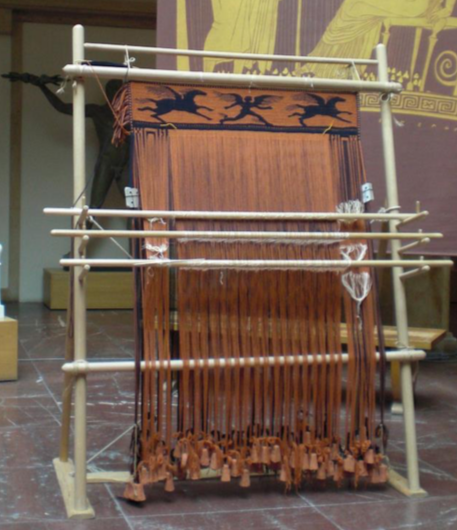
\includegraphics[scale=0.75]{loom}
\end{center}

Importantly, this method requires a starting/heading band to be made and then placed at the top of the warp-weighted loom. This starting band, which can be only a few threads, is made on a separate, horizontal loom. The weft threads of this initial weaving become the above-described warp threads of the warp-weighted loom. Thus, once the the warp-weighted loom is set up, many facets of the weaving-to-be are already predetermined, including the web's length (the width of the loom) and the web's width (the length the warp threads).\footnote{ Still, ``the warp-weighted loom is a very flexible device ... it is possible to detach and rearrange the weights at any time, to change the direction of the warp, to change the heddles and the rhythm of warp-lifts, and to combine different types of weave'' (Harlizius-Kl\"{u}ck \& Fanfani 2016: 73). I wish to emphasize, though, that a maximum set of dimensions for a given web is entailed by the setup described here, at least without the stitching of a separately weaved cloth. Again, the heading band ``provides the preliminary operation of ordering a textile ... that predicts the measure, and often the quality, density, and the numbers of warp threads for the whole weave'', per Harlizius-Kl\"{u}ck \& Fanfani (2016: 74). } Even before this, ``many decisions have to be made ... [namely] on yarn thickness, on quality and length, ... [on] the distribution of coloured threads, [on] the number of threads necessary to achieve certain patterns''.\footnote{ Harlizius-Kl\"{u}ck \& Fanfani 2016: 71.} Knowledge of strict arithmetic structures is requisite in planning a particular weave's pattern.\footnote{ ``Knowledge of divisibility rules and number features such as odd, even, prime, relatively prime and knowledge of least common multiples and greatest common divisors was necessary to weave the elaborate patterns we see in the visual representations'', per Harlizius-Kl\"{u}ck \& Fanfani (2016: 74).} These structures have a distinctively dyadic character: the binary both of warp/weft and of the separate warp threads themselves.\footnote{ Harlizius-Kl\"{u}ck \& Fanfani (2016) argue that weaving is a source for dyadic arguments in other domains, such as geometry and philosophy.}
 
Recent scholarship has made it clear that it's worth taking seriously the notion that weaving metaphors in literature operate over literal weaving mechanics. In other words, the weaving metaphors described in Section 2.1 are often times neither vague nor general, nor based only on abstract links; instead, the metaphors can make reference to precise weaving structures. Notably, Tuck (2006) has linked poetic metrical structures qua mnemonic devices to the literal weaving of varying patterns.\footnote{ Unfortunately, Tuck doesn't provide any explicit mapping between mnemonic song and textile.} Nosch (2014) has more directly claimed that certain metrical structures correlate to particular dyadic warp patterns.\footnote{ E.g., a dactyl (long-short-short, \={} \u{} \u{}) is related to a warp thread pattern front-back-back (+ -- --); this is admittedly somewhat speculative on Nosch's part.} 

Crucially for the present paper, Harlizius-Kl\"{u}ck \& Fanfani (2016) have shown that the heading band is a fundamental and productive concept in weaving-poetry metaphors. Specifically, the idea that a poetic work is an explicit arrangement (κόσμος) with limits, a border (πεῖραρ), ``rests on the construction of the songs' foundation ... [and] the beginning as a starting front of the poem bears special relevance to archaic Greek poetics''.\footnote{ Harlizius-Kl\"{u}ck \& Fanfani 2016: 85. See also Nagy 2010ab and Bergren 1975.} Furthermore, this poetic \textit{kosmos}, they claim, relates to ring (ABA) structures, though the precise mapping from weaving to literary structure is obscure here.\footnote{ See also Bergren 2008 and the discussion at the end of the next section.} Following Nagy (2010b), Harlizius-Kl\"{u}ck \& Fanfani (2017), claim the προοίμιον, defined as `starting thread', functions as a heading band of epic verse insofar as it links the recitation of the verse to the occasion of that recitation (some festival to a particular god). Therein, the \textit{prooimion} delimits the content of the song/performance (the οἴμη,  `thread') to follow; though, again, the precise mapping is obscure. An important question remains here: Can verse/poetry be delimited by a \textit{prooimion} in the same way a weave is delimited by a heading band? I will show below that this is a problem that Homer tries to tackle with Penelope's weaving trick.

Finally, Harlizius-Kl\"{u}ck \& Fanfani (2017) describe ῥάπτειν (`to stitch') as something altogether different than the common translation `to sew'. According to them, ῥάπτειν is used ``not for sewing thread running parallel to the border without taking into account the structure of the joint fabrics, but by carefully inserting the loose threads into the structure''. Therein, the joining of completed fabrics comprises ``various techniques ... ranging from plaiting a very different structure with the threads provided by the larger fabric ... to weaving an additional band where the loose warp threads from the weave are integrated step by step into the new fabric as weft''. What I wish to emphasize here is that stitching in these cases still operates on otherwise completed webs and is not simply a continuation of the same weaving processes of the first web: either an explicit 90-degree turn or a change in structural type altogether is necessary.

\section{\textit{Humnos} structure (Nagy 1996ab, 2010ab)}


A number of works have described how the weaving metaphors might operate on a literary level, many of which utilize Penelope's web in particular. Most of these works focus on how weaving has implications on higher-order literary questions, most notably literary theory (i.e., theories of signifiers and signifieds), gender dynamics, and political implications. These latter works will be dealt with directly, insofar as they are relevant, during the discussion of Penelope's trick, below. The purpose here is to detail how the weaving metaphors are used as a framework for producing literary works, for which Nagy (1996ab, 2010ab) provides the most thorough and explicit framework. 

\subsection{Basic Framework}

Despite the time gaps and minor divergences between Nagy's various works, in general he seems to consistently posit the same basic framework for how weaving terms are manifest in (pre-Homeric, Homeric, post-Homeric) Greek poetry.\footnote{ This framework, being scattered within and between various works, is somewhat difficult to reconstruct in precise ways, as it contains a number of (at least) logical lacunae. I discuss some of these logical issues below.} The diagram below collates and summarizes the basic structure of a ὕμνος (\textit{humnos}, `hymn, song') as reconstructed by Nagy in surveying the \textit{Iliad}, the \textit{Odyssey}, the \textit{Homeric Hymns}, and various other post-Homeric authors (notably Pindar, Theocritus, Callimachus, and Apollonius of Rhodes). The \textit{humnos}, according to Nagy, is one of the basic schemata in/through which Homeric poetry is constructed.\footnote{ By `Homeric' here and throughout I'm referring to the broad definition given by Nagy that includes the two Homeric epics we have today, as well as Nagy's reconstructed forms of the Homeric Cycle / Homeric Hymns and of Orphic traditions that, prior to Panathenaic regularization, were also considered Homeric. The \textit{humnos}, according to Nagy, over time becomes illicit for regularized epic, but is prevalent in the earlier, pre-regularized forms. Despite this, the same basic structure of the \textit{humnos} below is still relevant, in differing ways, for post-Homeric (e.g., Pindar) and post-regularization (e.g., Callimachus) poetry.}

\newpage
\begin{singlespacing}
\ex. structure of a \textit{humnos} according to different descriptors

\begin{small}
\begin{center}
\begin{tabularx}{\textwidth}{
|>{\centering\arraybackslash}X
||>{\centering\arraybackslash}X
||>{\centering\arraybackslash}X
||>{\centering\arraybackslash}X
|
}

\multicolumn{1}{l}{a. formal terms} & \multicolumn{1}{l}{b. signal words} & \multicolumn{1}{l}{c. general functions} & \multicolumn{1}{l}{d. section examples} \\
\hline
\textit{prooimion} & ἄρχεσθαι + genitive & opening `thread' = \par perfect beginning & \\

... & ... & ... & \textit{Homeric Hymns} \\
\cdashline{1-3}
\textit{metabasis} & χαίρε(τε) [divinity]  ... \par ἐγὼ αὐτἀρ & move ahead \& shift forward (to new topic/form) = perfect transition & Demodokus' 2nd song (?) \\
... & ... & ... &  \\
\hline
epic / choral / other genre & (optional: κλέα and/or ἔργα) & the hymnic consequent = perfect continuation & Homeric Epic \\
... & ... & ... & Homeric Cycle \\
\cdashline{1-3}
\textit{telos} & (optional, varying location: Διὸς βουλή) & plan of Zeus = perfect end & Demodokus' 1st/3rd songs \\
\hline

\end{tabularx}
\end{center}
\end{small}
\end{singlespacing}

\noindent \hfill \par

The (a), (b), (c), (d) structures each represent one and the same \textit{humnos} in different terms: (a) shows the formal terminology for each section of a \textit{humnos}; (b) shows the words that signal each section within a given \textit{humnos}; (c) shows Nagy's descriptions of each section's general function; (d) shows extant textual genres that represent (though in some cases in different ways) these sections. Though there are some complications, discussed below, this is the minimal structure for a \textit{humnos}. In sum, a \textit{humnos} begins with a \textit{prooimion}. This beginning shifts into the `hymnic consequent' via a \textit{metabasis}, the latter of which can be used to create otherwise illicit gaps in a given narrative. The hymnic consequent can be epic poetry\footnote{ Again, in a general sense that's not tied to the Homeric poems as we have them.}, but the hymnic consequent can also be, at least hypothetically, a different genre of song, like choral.

\subsection{Weaving Operations/Implications}

The craft of weaving is a motivating metaphor for the creation of a \textit{humnos}. As stated above, Nagy links the word ὕμνος (`hymn, song') to ὑφαίνειν (`to weave'), indicating that the act and product of creating a \textit{humnos} is, at least in a general sense, metaphorized as the act and product of creating a web. The creation of poetry in general it seems, but especially of Homeric epic in particular, is further characterized by ποικίλλειν (`to pattern-weave'), i.e., by making a web that is ποικίλος (`variegated, varicolored').\footnote{What this description actually characterizes is somewhat unclear.} This `variegated web' metaphor for poetry goes all the way back to the Bronze age.\footnote{ See Nagy 2010b: 291-305, which includes how bronze-/metal-working and ceramic-ware is also made to be `variegated'.} Abstractly, Nagy (1996b: 60) understands ποικίλος as applied to poetry to mean that poetry is characterized by `continuity through variety', and ``the essence of this craft of pattern-weaving ... is variety itself and the pleasurable beauty to be found in variety''.\footnote{ See also Nagy 2010b: 305.} A single song, then, or at least an epic song, is not uniform in its composition but is made of a variety of parts.\footnote{ Again, it's not clear what exactly the delineated parts of a given song are, to be discussed below.} Furthermore, poetry as `pattern-weaving' gives poetry a certain ``prestige'' as an intricate art,\footnote{ Nagy 2010b: 300.} a status eventually bolstered by the fact that the archetype of `pattern-weaving' becomes Athena's ritual \textit{peplos}, which itself was made by master artisans.\footnote{ Nagy 2010b: 280.}

Nagy (2010a: 280) characterizes a \textit{humnos} as having a certain perfect `continuity' or `fluency': ``the hymnos is ... a song that functions as a connector, a continuator''. Thus, a \textit{humnos}, including, in some way, Homeric poetry, is characterized by ``starting with a perfect beginning, continuing with the perfect sequence, and finishing off with the perfect \textit{telos} ...  the most perfect expression of this perfection is the word \textit{humnos}''.\footnote{ Nagy 2010b: 313.} As the diagram indicates, a perfect $\langle$beginning, sequence, ending$\rangle$ corresponds to a perfect $\langle$\textit{prooimion}, \textit{metabasis} + (set of?) epic(s), \textit{telos}$\rangle$. The perfection of a \textit{humnos} is derived from the god in whose honor the \textit{humnos} is sung, and that god becomes both source and subject of the \textit{humnos}.\footnote{ I.e., ``the source of the perfection is the god [here, Apollo] as the subject of the \textit{humnos}'' (Nagy 2010a: 197), while ``Zeus is the ultimate source for any \textit{humnos}'' (Nagy 2010b: 101).} Apollo and the Muses are originally the paradigm cases for gods that produce perfect \textit{humnoi}, later to be replaced by Zeus as ultimate source. Since the \textit{prooimion} is a sub-part of a \textit{humnos}, the perfect beginning is a defining characteristic of the \textit{prooimion} itself and of the \textit{humnos} in its totality.\footnote{ ``Both \textit{humnos} and \textit{prooimion} convey the poetic idea of the authoritative  beginning that makes continuity possible. But the word \textit{humnos}, unlike \textit{prooimion}, refers not only to the start of the continuum but also to the continuum itself'' (Nagy 2010a: 312).} Finally, the \textit{telos} for Nagy is tantamount to the Διὸς δ’ ἐτελείετο βουλή (`the plan of Zeus being completed'), which refers to the conclusion of the Trojan War via the \textit{Iliou Persis} (`the sack of Troy').

The \textit{prooimion} of a \textit{humnos} is the beginning of this perfect sequence, which also happens to fit into the poetry-as-weaving metaphor. Specifically, as mentioned above, the \textit{prooimion} is derived from the root \textit{-oim-}, `thread'. By invoking some god, then, the \textit{prooimion} becomes the `starting thread' of this perfect sequence, that, within the sequence, gets continued perfectly until its proper end. Nagy extends the `thread' metaphor from the \textit{prooimion} to the \textit{metabasis} of the \textit{humnos}; that is, he metaphorizes μεταβαίνειν (`moving ahead') as `threading one's way from one point to another'.\footnote{ Nagy 2010a: 330.} It's important to note, as Nagy is not clear on this, that μεταβαίνειν does not by itself have any particular connection to `thread'; Nagy instead deduces a `thread' connotation based on the context of the \textit{humnos}. Again, `threading' seems most naturally considered a particular part of weaving in general, insofar as weaving utilizes, and a web is made up of, threads. In particular, the \textit{prooimion} ostensibly functions as the `heading band' of a particular \textit{humnos}. It will be useful in the discussion of Penelope's web to maintain this part-whole (i.e., thread-weaving) distinction and to not unilaterally subsume them both into the general ``metaphorical world'' of ``the making of fabric'' as Nagy (2010a: 229 ff.) does.

I will pause here to note a problem that has already arisen in the weaving metaphor as postulated by Nagy. While the \textit{metabasis} can be provided a thread-based interpretation, there is, unlike the \textit{prooimion}, no particular literal basis in thread for the \textit{metabasis}. While the \textit{prooimion} can be thought of as a `heading band', no such explicit structural correlate exists for the \textit{metabasis}. Furthermore, Nagy never even tries to work the \textit{telos} of a \textit{humnos} into the thread metaphor, nor is it clear in what way the \textit{telos} of a \textit{humnos} would be characterized as a `thread'.\footnote{ Nagy does, as has been shown, say the perfect beginning leads to a perfect end and that the beginning and middle are `threads', but he does not explicitly characterize the end as `thread'. Malsov (2012) makes an even stronger case by claiming that even the \textit{prooimion} didn't, in Homeric times, signify an opening to a poetic work.} This is an important divergence from the actual mechanics of weaving. While the heading band of a web, per the above discussion, implies the dimensions, and therefore the `end' of the web, this implication does not arise in any clear sense for the \textit{prooimion} of a \textit{humnos}.\footnote{ Nagy does talk about what the \textit{telos} of a \textit{humnos} is, to be discussed shortly.} A question then remains: In what way, if at all, must a song end if it's characterized by weaving and by starting with a `thread'? I will return to this problem below.\footnote{ Harlizius-Kl\'{u}ck and Fanfani (2016: 90) try to give a more concrete role to the \textit{prooimion}, saying that ``the \textit{hymnos/prooimion}, just like the warp which is governed by the starting border, developed different patterns and narrative motifs throughout the rhapsodies performed by the competing singers''. Even if this is the case, it doesn't answer the problem of how a \textit{prooimion} could entail any particular ending given some subset of chosen themes.}

\subsection{Stitching Operations/Implications}

\textbf{The Problem}

As it stands, though, a more superficial problem pertains to Nagy's deployment of a separate fabric metaphor, namely that of `stitching'. As said above, the activity of the \textit{rhapsodes} is etymologically defined as `those who stitch songs together', an etymology that Nagy (2010ab) exploits. Nagy therein also derives the name `Homer' itself from a root that means `to join', primarily in the domain of carpentry, but Nagy argues that the tradition of Homer conceives of the bard as a `joiner of song'. I.e., the names for Homer and for Homeric performers both connote essentially the same thing, that of combining songs. What type of song these joiners join, however, is difficult to parse from Nagy's analysis, as that type seems to change depending on whatever argument Nagy is deploying in the moment. Again, the problem is to decipher what poetic entity `stitching' applies to.

Before detailing and attempting to solve that problem, I will very tersely recap the pertinent parts of Nagy's argument. Nagy claims that Demodokos' three songs in book viii of the \textit{Odyssey}, Odysseus' epic in book ix-xii, and the mention of Demodokos singing in book xiii are all part of one continuous \textit{humnos}, a ``single ongoing narrative'' in the context of a \textit{dais}, a ritual feast, for Zeus.\footnote{ Nagy 2010a: 326. See also Nagy 2010b: 79-102.} Zeus is the overseer of the festival and thereby of this set of hymns, and Zeus thus acts as the perfect source of these hymns. Nagy relates the various songs within this giant \textit{humnos} to different historical types, in order from oldest to newest form: Demodokos' second song represents Orphic poetry and the \textit{Homeric Hymns}; Demodokos' first, third, and final songs represent the Homeric Cycle; Odysseus' song represents Homeric epic as we have it today.\footnote{ Nagy 2010b: 79-101, especially 89. In fact, there ``is a competition between preregular and regular epic'' (Nagy 2010b: 96).} The first and third songs of Demodokos feature \textit{prooimia} implicitly to Zeus, as well as \textit{metabases}.\footnote{ The status of ``implied'' is unclear. Nagy wants to distinguish between Demodokos' songs and Odysseus' song as preregular and regular epic, respectively. However, both Demodokos' songs and Odysseus' song are (seemingly, at least) in Nagy's third category of \textit{prooimia} `implicitly' to Zeus. What he might mean is that, for Demodokos' songs, it is implied by the outer narrative that the \textit{prooimia} are explicitly to Zeus in those songs themselves, but this would be a strained reading. Finally, it's not clear why Nagy doesn't consider the openings to our extant \textit{Iliad} and \textit{Odyssey} to have implicit \textit{prooimia} to the Muses, even though this would seem possible based on his own criteria (Nagy 2010b: 119).} The first song of Demodokos (seems to) implicitly include several \textit{prooimia} and \textit{metabases} internal to itself, as well. The second song of Demodokos also features a \textit{prooimia} to Ares and Aphrodite, both subordinate to Zeus. These \textit{prooimia}/\textit{metabases} serve as the mechanics for linking those three songs into one \textit{humnos} and further characterize them as pre-regularized Homeric epic. On the other hand, the transition to and from Odysseus' song features no formal or explicit hymnic mechanics, like regularized Homeric epic.\footnote{ Nagy 2010b: 102.} Finally, the `plan of Zeus' as \textit{Iliou Persis} is the necessary end of Demodokos' third, and therefore also of his first, song; this end is superseded by Odysseus taking up the helm and singing his own epic, as regular overtakes pregular epic.

Already two problems arise in Nagy's system. First, it's not clear in which cases \textit{prooimia} and \textit{metabases} are necessary for connection, in which they're optional, and in which they're illicit, nor, relatedly, is it fully clear what sorts of textual objects (in terms of completeness and genre) are connected by such devices. On the one hand, Nagy (2010a) claims that separate songs of a pre-regularized epic cycle require \textit{prooimia} and \textit{metabases} in order to be connected to each other. The implicit \textit{prooimia} within Demodokos' first song that, implicitly connect different sub-songs within that first song, is a primary driver in Nagy's argument.\footnote{ Nagy (2010a: 332) says that ``without this new \textit{prooimion} there can be no metabasis, and without the metabasis there can be no new performance of epic. The epic of the third song about the end of the Trojan War cannot simply follow the epic of the first song about the beginning of the war.''.} On the other hand, Nagy also claims that these \textit{prooimia}/\textit{metabases} are not necessary for the same set of preregular songs.\footnote{ I.e., a diachronic argument wouldn't solve the problem. Nagy (2010b: 103) claims that ``It does not follow ... that each restarting of epic requires a distinct hymnic \textit{prooimion}. ... [A] hymnic \textit{prooimion} is not obligatory for restarting or even starting a given epic---provided that Zeus happens to be the implied hymnic subject who authorizes that epic.''. Zeus, Nagy claims, is the implied hymnic subject of the songs for which \textit{prooimia} (and \textit{metabases}) were necessary (see the above footnote) to connect the songs within the first and between the first and the third songs of Demodokos. Again, the status of ``implied'' is itself unclear.}

Second, as noted above, Zeus is supposed to be the ultimate overseer and source of any possible \textit{humnos}, including Demodokos' set of songs.\footnote{ At least by the time of the Homeric Cycle, which comprises Demodokos' songs.} However, the `plan of Zeus', the \textit{Iliou Persis}, is, more specifically, a (potential) characteristic of epic. Epic, again, is only an optional hymnic consequent. A disjunct thus occurs between two levels of hymnic phenomena for which Nagy invokes the necessity of Zeus: the hymn itself and an optional sub-part of the hymn. This makes dubious the hymnic, though perhaps not epic, necessity of the `plan of Zeus', which further heightens the problem noted above as to how to predict the perfect \textit{telos} of a \textit{hymnos} from the perfect \textit{prooimion}. Nagy (2010b: 95) says that ``either it [Demodokos' third song] will continue in the ways of a poetic form exemplified for us by the \textit{Homeric Hymns} [Demodokos' second song] or it will recycle back to ... the first song of Demodokos'', which indicates that Demodokos' third song, and therefore the `plan of Zeus', need not strictly have ever been uttered, despite Demodokos' first song. If Nagy's claim here is that Demodokos could continue to sing \textit{Homeric Hymns} as long as, eventually, he sings the `plan of Zeus', this would mean either that epic is a necessary hymnic consequent or that the `plan of Zeus' is not strictly relegated to epic; both of these conclusions are denied by Nagy elsewhere. Thus, two levels of Zeus' power obtain: a) a higher-order one by which Zeus oversees \textit{hymnoi} in general; b) a lower-order one (because epic is a subset of \textit{hymnoi}) in which Zeus determines the outcome of epic. The problem as to how to derive the hymnic \textit{telos} remains.

It's now possible to discuss the basic problem noted above as to what phenomena `stitching' refers to. The ultimate cause of this problem is that Nagy elides the mechanical difference between `stitching' and `weaving'. Recall that `stitching' and `weaving' \textit{per se} are separate processes, per my discussion above on Harlizius-Kl\"{u}ck \& Fanfani (2017). This difference obtains even if it's the case that one or more woven webs are `stitched' together using the threads of those same webs and that the resulting set of webs is then itself called one web. The warp-weighted loom is not used in the same way for `stitching' as the shed-counter-shed process of weaving itself. 

Nagy (1996b: 75), before the full formulation of $\langle$\textit{prooimion}, \textit{metabasis}, hymnic consequent, (\textit{telos})$\rangle$, originally claims that ``the stitcher, one who sews together pieces of fabric already woven, is a master craftsman ... fashioning something altogether `new' ''. However, that picture of the stitcher is based on an outdated etymology that derives \textit{prooimion} from a root meaning `to sew' '',\footnote{ Nagy 1996b: 63-64.} which would provide a clear connection between \textit{prooimion} and the \textit{rhapsode} qua stitcher. However, Nagy (2010a) later derives \textit{prooimioin} from a root meaning `thread', which is now a more accepted etymology. Nagy (2010a: 231) then claims, from the new etymology, that ``Such etymological connections [i.e., that \textit{prooimion} and \textit{humnos} relate to weaving] with the metaphorical world of making fabric are parallel to the poetic connection of the \textit{prooimion} of Zeus with the overt metaphor of \textit{rhapta epea} ‘stitched-together words’ in Pindar’s Nemean 2, which in turn is connected with a latent metaphor embedded in the etymology of the word \textit{rhapsoidos} ‘rhapsode’, a compound formation composed of the morphological elements \textit{rhaptein} ‘stitch together’ and \textit{aoide} ‘song’.''. The precise mechanical connection between `stitching' and `weaving', though, he does not elucidate, nor is still it etymologically apparent; a ``metaphorical world'' is not explanatory therein. Similarly, Nagy (2010a: 314-315) claims that ``the weaving of a web is a process of making connections'', which seems more apposite to `stitching' but is in any case not even descriptive.

Similarly, Nagy (2010b: 324) connects the `relay performances' of a series of Homeric \textit{rhapsodes} to a passage of Cicero that indicates that ``a weaver may finish a sequence of weaving only to restart it later in a new sequence''. The `relay performance' is supposed to represent `stitching', but the Cicero passage, per Nagy himself, uses words meaning `thread' (\textit{orsus}) and `to weave' (\textit{(con)texere}), and Nagy offers no explicit mapping between the two metaphors. Moreover, the Cicero passage indicates that the weaving objects worked by each \textit{rhapsode} are individually incomplete and that the \textit{rhapsodes} together weave one complete web. This characterization is completely at odds with Nagy's (1996b: 65-66) claim that \textit{rhapsodes} combine ``many and various fabrics of song ... each one already woven''. This earlier claim may be over-ridden, for Nagy, by the later claim. Still, the implication from the Cicero passage is clearly that, if `stitching' is `thread'-based, `stitching' occurs within a given \textit{humnos} and that the particular \textit{humnos} being worked on is explicitly incomplete. The entire explication of the \textit{Odyssey} book viii and Nagy's insistence that each \textit{humnos} is complete in-and-of-itself, however, seem to indicate that `stitching' would be between separate and complete (sub)-\textit{humnoi}. I will attempt to elucidate the contradictions more clearly by going through logically distinct, according to Nagy's system, cases as to the potential relevant phenomena for `stitching'.

\noindent \hfill \par
\noindent \textit{Case 1: `stitching' applies to the} humnos

Nagy's conflation of weaving and stitching implies that poetic `stitching' targets, in some sense, \textit{humnoi}. Recall that, apart from `stitching', only one set of mechanics are given for \textit{humnoi}, comprising the \textit{prooimion}, \textit{metabases}, etc.

\noindent \hfill \par
\noindent \textit{Subcase 1.1: `stitching' occurs within one} humnos

If `stitching' occurs within a \textit{humnos}, it must refer, at least in part, to the use of hymnic mechanisms like the \textit{prooimion}, which would be not only redundant but also, as has been shown, etymologically infelicitous. There is, furthermore, no mechanism left for the combination of various \textit{humnoi}, which must be possible given Nagy's discussion of the \textit{Odyssey} book viii. This option seems to make very little sense.

\noindent \hfill \par
\noindent \textit{Subcase 1.2: `stitching' occurs between} humnoi

This case will ultimately prove the basis for my solution below, but some difficulties remain. According to Nagy, each \textit{humnos} is notionally perfect. Nagy also takes a set of \textit{humnoi} as one \textit{humnos} of the same kind as its parts, which means this super-\textit{humnos} must also be notionally perfect. Taken strictly, this amounts to a competition between sequential \textit{prooimion} and, by extension, sub-\textit{humnoi} within a given super-\textit{humnos}. Supposedly, the first \textit{prooimion} and \textit{humnos} would reign, but there is no necessary reason for that to be the case. Nagy (1996b: 66) does call this a ``paradox'', but this is based on the overridden etymology for \textit{prooimion} as `to sew'. This case contradicts the Cicero formulation from above, since it implies that act of `stitching' operates on already complete webs.

\noindent \hfill \par
\noindent \textit{Case 2: `stitching' applies to epic}

The etymology of `Homer' and \textit{rhapsode} suggest that `stitching' should apply specifically to epic. Epic seems fundamentally to be a subpart of a \textit{humnos}. However, Nagy also sometimes talks about epic as overriding some set of \textit{humnoi}. This is most notable, per above, when the hymnic mechanisms are described as combining Demodokos' first and third songs and when the epic `plan of Zeus' is therein described as overriding even the non-epic second song of Demodokos. Similarly Nagy (2010a: 312) says that ``the \textit{humnos} is the sequencing principle that connects with epic, then extends into epic, and then finally becomes epic itself'', which potentially implies that epic becomes the overriding genre. I take both cases below.

\noindent \hfill \par
\noindent \textit{Subcase 2.1: epic is a subcategory of the} humnos

\noindent \hfill \par
\noindent \textit{Subsubcase 2.1.1: epic uses hymnic mechanisms for `stitching'}

Since epic is a subpart of \textit{humnos}, this would entail the problems of both Subcases 1.1 and 1.2, making it untenable.

\noindent \hfill \par
\noindent \textit{Subsubcase 2.1.2: epic doesn't use hymnic mechanisms for `stitching'}

If epic doesn't use hymnic mechanisms for `stitching', it remains to be detailed what subparts of epic are being `stitched'. Furthermore, Nagy only uses hymnic mechanisms to describe the combination of epic songs. 

\noindent \hfill \par
\noindent \textit{Subcase 2.2: epic is, or can be, a supercategory of the} humnos

That different songs of epic can be combined using hymnic mechanisms implies, per above, that epic can be a supercategory of \textit{humnos}. This means, because epic is also a subcategory of \textit{humnos}, that epic is a subcategory and supercategory of itself. This is either trivially true (by the reflexive property of sets, see Case 3, below) or an absolute contradiction (assuming that the epic is, in particular, a proper subset of \textit{humnos}). In any case, if the second song of Demodokos, which Nagy explicitly says is not epic, is part of the \textit{humnos} of book viii, it makes little sense to call that \textit{humnos} `epic' by Nagy's own account, accept by coercion.

\noindent \hfill \par
\noindent \textit{Case 3: `stitching' applies to both epic and} humnos

If \textit{humnos} and epic can refer to the same object according to formal features, it would make little sense distinguishing them so harshly in the first place. All the problems above would still obtain, regardless. A diachronic argument could be made for this case, as I will below. Nagy, though, doesn't do so in any explicit terms for the \textit{humnos}-epic relationship, though he hints at it, and the two types must still be formally distinguishable in some way for any such diachronic argument to work.

\noindent \hfill \par
\noindent \textbf{Solution}

As mentioned, the base of the solution for tying all these structures together is Case 1.2, above. First, `weaving' operates within \textit{humnoi}, creating a completed \textit{hymnos}, and `stitching' operates on sets of (`woven') \textit{humnoi}, namely to combine them. Thus, `stitching' operates on otherwise complete hymnic objects, similar to some of Nagy's (1996b) claims. The Cicero passage, and `weaving' operations on incomplete objects in general, then, refer to within-\textit{humnos} weaving and not to the `stitching' of songs. Furthermore, a set of \textit{humnoi} connected by `stitching' might itself be called a \textit{humnos}, but, crucially, unlike Nagy's formulation, this super-\textit{humnos} is not subject to the same metaphor as each sub-\textit{humnos} and is definitionally only a \textit{humnos} by metonymy.\footnote{ Nagy (2010a: 231) seems to approach this conclusion, saying ``By metonymy, the \textit{humnos} includes the rest of the performance, proceeding sequentially all the way to the conclusion of the whole performance'', but this is not definitional and is overridden by his conflation of weaving and stitching.} 

As for epic, this is definitionally a subpart of a single \textit{humnos}, as much of Nagy's analysis suggests. As a subpart, epic is subject to being `woven' and to Cicero's incompleteness formulation. This sense of epic would actually fit well with Nagy's diachronic argument with regard to the development of epic. Namely, it could be the case that, just as a set of \textit{humnoi} can be a called ``a \textit{humnos}'', so a set of epic \textit{humnoi} (defined as having epic hymnic consequents), can be called ``an epic''.\footnote{ Recall that the `weaving' metaphor can be traced all the way back to Indo-European, but this is not the case for `stitching'.} If Homer later becomes historically associated specifically with epic,\footnote{ Per Nagy 2010a: 249, ``Homer was viewed as the notional author of all epic''.} Homer qua `stitcher' would simply be a particular case of a more general phenomena of `stitching'.\footnote{ Again Nagy (2010a: 210) seems to approach this, saying ``The figure of Homer himself can now be viewed as the sum total of his notionally perfect songs'', but it's difficult to parse the exact relation between \textit{humnos} and epic.} I diagram the solution below.

\ex. a set of \textit{humnoi}

\begin{tikzpicture}
\indent \draw (0,0) rectangle (4,2);
\node at (0.5,1) {\rotatebox[origin=c]{90}{\textit{prooimion}}};
\node at (1,1) {\rotatebox[origin=c]{90}{\textit{...}}};
\node at (1.5,1) {\rotatebox[origin=c]{90}{\textit{metabasis}}};
\draw [dotted] (2,0) -- (2,2);
\node at (2.5,1) {\rotatebox[origin=c]{90}{epic, etc.}};
\node at (3,1) {\rotatebox[origin=c]{90}{...}};
\node at (3.5,1) {\rotatebox[origin=c]{90}{(\textit{telos})}};
\node at (4.5,1){\rotatebox[origin=c]{90}{`stitching'}};
\draw (5,0) rectangle (9,2);
\node at (5.5,1) {\rotatebox[origin=c]{90}{\textit{prooimion}}};
\node at (6,1) {\rotatebox[origin=c]{90}{\textit{...}}};
\node at (6.5,1) {\rotatebox[origin=c]{90}{\textit{metabasis}}};
\draw [dotted] (7,0) -- (7,2);
\node at (7.5,1) {\rotatebox[origin=c]{90}{epic, etc.}};
\node at (8,1) {\rotatebox[origin=c]{90}{...}};
\node at (8.5,1) {\rotatebox[origin=c]{90}{(\textit{telos})}};
\node at (9.5,1){\rotatebox[origin=c]{90}{`stitching'}};
\node at (10,1){\rotatebox[origin=c]{90}{...}};
\node at (2,-0.5) {complete \textit{humnos} 1};
\node at (4.5,-0.5) {+};
\node at (7,-0.5) {complete \textit{humnos} 2};
\node at (9.5,-0.5) {+};
\node at (10,-0.5) {...};
\node [right] at (10.5,-0.5) {$\approx$ \textit{humnos}/epic};
\end{tikzpicture}


The solution here has the benefit of being relatively faithful to Nagy's system while avoiding contradictions, and also of maintaining the historical/mechanical differences between stitching and weaving.\footnote{ It also fits well with the description by Lord (1960: 94), as cited in Slatkin (1996: 226): ``Although the themes lead naturally from one to another to form a song which exists as a whole in the singer's mind with Aristotelian beginning, middle, and end, the units within this whole, the themes, have a semi-independent life of their own. The theme in oral poetry exists at one and the same time in and for itself and for the whole story.''.} Another implication arises that would be less apposite to Nagy, though. If a particular \textit{humnos} is supposed to have  a perfect \textit{telos}, this \textit{telos} definitionally can't operate outside that \textit{humnos}. As stated above, this makes it very unclear how a particular \textit{humnos}, especially a non-epic \textit{humnos}, can achieve its perfect \textit{telos}, since, unlike weaving proper, a \textit{prooimion} does not entails its own end. Similarly, it's also very unclear how a set of \textit{humnoi} can achieve any end, let alone a perfect one. The `plan of Zeus' is no help in this latter case, because nothing entails that any particular set of \textit{humnoi} must end with the \textit{Iliou Persis}.\footnote{ As in the case of our extant \textit{Iliad}, as even Nagy (2010b: 122) notes: ``Thus the expression \textit{Dios d’ eteleieto boulē} `and the Plan of Zeus was reaching its \textit{telos}' at verse 5 of \textit{Iliad} I presupposes a narrative framework that is far broader than the actual narrative that is getting under way in our Iliad. Zeus is in charge of that broader framework, but the epic plot of our Iliad cannot be explicitly equated with that framework.''. Even if the `plan of Zeus' is the maximum outer limit of possible epic narrative, this would by no means entail that that limit must in every case be reached. At least for some diachronic states of Homeric poetry, moreover, the \textit{Odyssey}, as Nagy (2010b: 102) notes, contradicts that premise, anyway. Nagy's (2010a) characterization of Homeric epic as ``linear'' fits this problem. Bergren (2008: 54) claims that it is, in fact, crucial that Zeus' plan exceeds the \textit{Iliad} itself, while also giving final authority not to Zeus but to the singing bards.} 


Two fundamental problems thus remain: i) how can a \textit{humnos} end; ii) how can a set of `stitched' \textit{humnoi} end.\footnote{ Felson-Rubin (1994: 151-2n9) implicitly invokes these two modes, though she doesn't derive it from a technical problem. She writes that ``images of weaving evoke not only the phenomenon of making the poem by weaving storylines into strands of plot; they also suggest what listeners experience as a final product: a dappled tapestry, a visible object''.} The analysis of Penelope's web, below, will show that these are problems that the \textit{Odyssey} is aware of and tries to solve. I'm going to characterize these two problems in abstracted formulaic terms in order to facilitate their discussion. I therein offer `equations' for weaving and stitching, respectively.


\ex. weaving equation
\a. ideal: \begin{math} \frac{1}{n} + \frac{2}{n} + ... + \frac{m}{n}, \; m = n \end{math}
\b. problem: \begin{math} \frac{1}{n} + \frac{2}{n} + ... + \frac{m}{n}, \; m > n \end{math}
\z. \z. 

\ex. stitching equation
\a. ideal: \begin{math} \frac{n_1}{n_1} + \frac{n_2}{n_2} + ... + \frac{n_m}{n_m}, \; \exists a \end{math} such that \begin{math} m \leq a \end{math}
\b. problem: \begin{math} \frac{n_1}{n_1} + \frac{n_2}{n_2} + ... + \frac{n_m}{n_m}, \; \neg \exists a \end{math} such that \begin{math} m \leq a \end{math}
\z. \z. 

Thus, weaving can be defined as an operation that creates one whole based on an indefinite number of sub-whole maneuvers (i.e., the back and forth of the weft).\footnote{ The symbol `+' here refers to simple concatenation, not to an arithmetic sum. I don't mean to imply that `weaving' or `stitching' could uniquely be abstracted from these equations, nor that any weaver, past or present, has anything like this in mind when weaving or stitching.} Problem arises if the numerator (the number of weft threads) exceeds that of the denominator (for a given thread width, the length set by the heading band). For a \textit{humnos}, which doesn't have a set length, this is a serious risk. Stitching, furthermore, can be defined as an operation that creates a set of completed woven materials, and this operation has a defined endpoint. Problem arises when no such endpoint exists. Again, for a set of \textit{humnoi}, which has no set length, this is also a serious risk.

It's also worth noting that Demodokos' first song as Nagy presents it now takes part in this double problem. Namely, Nagy claims, that the phrase ἂψἄρχοιτο (‘he would start again and again’) in book viii.90 indicates that Demodokos is starting, via \textit{prooimia}, various new hymns. If a pause in the performance can refer to something within epic, though, it's possible but not necessary that a set of hymns is indicated here. Demodokos first song, then, is ambiguous with respect to what is ``endless'' about Demodokos' first song, as Nagy (2010a: 323) says. Either one \textit{humnos} or a set of \textit{humnoi} could have a problem of endlessness.

\noindent \hfill \par
\subsection{Other Concerns}

I will quickly note two aspects of Nagy's argument that will be useful for analyzing Penelope's web. First, Nagy notes in several instances how the outer narrative of the \textit{Odyssey} book viii (i.e., the feast and Odysseus' reactions to Demodokos) come to supersede the inner narrative (i.e., the content of Demodokos' songs). In fact, Nagy (2010a: 343) says that ``the totality of narration in the third performance of Demodokos is achieved not directly but indirectly ... by way of the outer narrative that frames the third song''. Similarly, as Nagy notes, it is Alkinoos, in the outer narrative, that stops the potentially ``endless'' cycle of Demodokos' first song. Nagy stresses the ability of a \textit{humnos} to continue despite interruptions in the outer narrative. I would like to stress the inverse, however. It appears significant, I think, that the outer narrative consistently plays a role in stopping \textit{humnoi}. When discussing Penelope I will argue that this disjunction of levels of narrative is necessary to solve the two endlessness problems of \textit{humnoi}.

Second, Nagy (2010ab) consistently references the ring structures that occur in the \textit{Odyssey}, including in his analysis of book viii. He offers, though, little explanation as to why ring structures in particular are used in the particular ways they are used.\footnote{ That a ring structure would ``creat[e] ... the effect of a cycle'' is tautological (Nagy 2010a: 329). Similarly, it is not explanatory when Nagy (2010b: 92) says that ``there is a cycling back from one given point in the space of narration to an anterior point, picking up from there details that recycle forward into the ongoing narration, thereby augmenting it'', nor is the ensuing explanation. An explanation would show not just how a structure is used but why it is necessary.} Ring structure has long been a known feature of Homeric poetry, going back to the anciently known rhetorical device called ὕστερον-πρότερον (`the later (before) the earlier'), which describes the \textit{Odyssey's} frequent recourse to flashbacks.\footnote{ See Bassett 1920. Bergren (2008: 79-108) presents ring structure as constitutive of the \textit{Odyssey}'s narrative structure, forming the text's concern with νόστος 'return'.} The ὕστερον-πρότερον is formally the same as ABA structure when used temporally, since the `later' time is always returned to. Ring structure will also be pertinent to the Penelope discussion and the two endlessness problems described above.\footnote{ The implications I garner from the ABA structure, however, will be quite different from those of Bergren and others.} 

\section{Penelope's Weaving Trick}

\textbf{Brief Background}

Like weaving-based literature more generally, Penelope's weaving trick has garnered extensive academic treatment. Many of the modern treatments fall under the analytic-unitarian debate, based on the (relatively minor) divergences between the three instances of Penelope's trick in our extant \textit{Odyssey}.\footnote{ In book ii, xix, and xxiv, with varying lines. I'll provide these three instances shortly.} I will essentially shuffle the analytic debate aside and will assume that, however the final edition of the \textit{Odyssey} came to be, the three instances of Penelope's trick have some valid unified interpretation.\footnote{ This is in line with Nagy's general `evolutionary' approach to the Homeric corpus. Nagy (2004: 141), e.g., writes ``there is no way to decide which of any two or more `versions' is `the repeated version' ''. In any case, see Bona (1966) for most of the relevant issues.} 

The vein of my interpretation will be to treat Penelope's trick as a device for talking about poetics, broadly conceived. This vein has also been well-discussed in academic treatments, especially more recently, and for good reason. That the Odyssey is intentionally invested in showcasing its poetic self-conceptions and maneuvers is well-established independently of Penelope's weaving trick.\footnote{ See, e.g., Slatkin (1996) and Clayton (2004: 1-20) for summative expositions. As Bouvier (2014: 713) notes, even Aristotle commented on the robust meta-poetic qualities of the \textit{Odyssey}.} Furthermore, as has already been discussed extensively, weaving and related crafts provide fundamental metaphors for poetic production, a fact that is also independent of Penelope's weaving trick. Thus, Penelope's trick, among the most explicit and extended instances of the act of weaving in the Homeric corpus, is ripe for culling an understanding of Homeric poetics.\footnote{ E.g.: Katz 1991; Slatkin 1996; Felson-Rubin 1994; Papadopoulou-Belmehdi 1994; Clayton 2004; Bouvier 2014. Scheid and Svenbro (1996: 111-130) deny that Homer applies the weaving metaphor to his own craft, but Nagy (2010a) refutes this well. Kruger (2001: 82) also denies that Penelope is representative of Homeric poetics, but her argument is tautological.} Hence, Penelope is justifiably named the ``weaver par excellence''.\footnote{ See, e.g., Nosch 2014: 93, but any Google search for ```Penelope' `weaver par excellence'\nospace'' will provide numerous examples. The name `Penelope' is sometimes claimed to derive from πήνη (`thread'), though this is far from certain, and Beekes (2009) rejects it. See West 1990 for a discussion.}

However, scholarship that derives (some subset of) Homeric poetics from Penelope's trick are often too distended from precise weaving mechanics to make robust claims. Therein, the fact of the weaving metaphor \textit{per se} is taken as sufficient for undergirding higher-order interpretations. Penelope's trick then becomes a model for, in sum, some conception of the endlessness, or unendedness, of poetic activity, often without sufficient support.\footnote{ Clayton (2004) is the clearest example of this.} At least on a surface level, the fact that Penelope's trick does not strictly continue into infinity makes that line of interpretation difficult, though some try to include it.\footnote{ Again, see Clayton 2004. Kruger (2001) considers it ongoing since it is categorically distinct from the larger work.} In any case, to put it abstractly, these interpretations uncover a poetics of discrete infinity from the Penelope story, though that interpretation is not precisely grounded in textual specificities.

I will also claim that Penelope's weaving trick implies a discrete infinity as a potential structure for poetic activity. However, this structure is ultimately rejected by the \textit{Odyssey}: discrete infinity cannot be a basis for Homeric verse as we have it.

\subsection{ The Text of Penelope's Weaving Trick}

Penelope's weaving trick occurs in three places in the \textit{Odyssey}: one each in books ii, xix, xxiv. The first instance is narrated by the suitor Antinoos to Telemachus during an Ithacan assembly, the second by Penelope herself to Odysseus disguised as a beggar, the last by the suitor Amphimedon to Agamemnon in the underworld. In all three, Penelope is directly quoted giving a speech to suitors in which she describes her desire to finish a funeral shroud for Odysseus' father, Laertes, before conceding to wed one of the suitors. This speech is essentially identical in all three versions, minus pronominal and agreement changes. The lines immediately preceding and proceeding Penelope's speech are also quite consistent in all three versions, though there are important differences. I provide the Greek and English texts below,\footnote{ The Greek text is taken directly from the Loeb online edition. Translations are mine unless otherwise stated, with input from the Loeb translation and Wilson's (2018) translation.} divided according to category (see the following page).

In sum, Penelope, known for her cunning and being pressed to wed by many suitors, requests to delay marriage until she has finished a funeral shroud for Laertes. Penelope, to delay the wedding, contrives to weave the shroud by day and unweave it by night. One or several of Penelope's maids tattles on her and the suitors force her to complete the web. Importantly, then, Penelope has very recently finished Laertes' funeral shroud by the time Odysseus lands in Ithaca,\footnote{ How immediate this is varies between versions, but not, I think, to significant effect.} having pulled the trick off for three years.\footnote{ See West (1990: 137-138) for the purported, ultimately trivial, internal time discrepancy and other timeline-related concerns.}

\begin{sidewaystable}

\begin{singlespacing}

\ex. Greek text


\begin{tiny}
\begin{center}
\begin{tabularx}{\textheight}{
|c
||c
:>{\lefting\arraybackslash}X
||c
:>{\lefting\arraybackslash}X
||c
:>{\lefting\arraybackslash}X
|
}

\multicolumn{1}{l}{} & \multicolumn{2}{l}{a. ii.85-114} & \multicolumn{2}{l}{b. xix.130-161} & \multicolumn{2}{l}{c. xxiv.120-152} \\
\hline
\parbox[c]{}{\multirow{6}{*}{\rotatebox[origin=c]{90}{pre-context}}} & 85 & “Τηλέμαχ᾿ ὑψαγόρη, μένος ἄσχετε, ποῖον ἔειπες & 130 & "ὅσσοι γὰρ νήσοισιν ἐπικρατέουσιν ἄριστοι, & 120 & τὸν δ᾿ αὖτε ψυχὴ προσεφώνεεν Ἀμφιμέδοντος· \\
& 86 & ἡμέας αἰσχύνων· ἐθέλοις δέ κε μῶμον ἀνάψαι. & 131 & Δουλιχίῳ τε Σάμῃ τε καὶ ὑλήεντι Ζακύνθῳ, & 121 & “Ἀτρεΐδη κύδιστε, ἄναξ ἀνδρῶν Ἀγάμεμνον, \\
& 87 & σοὶ δ᾿ οὔ τι μνηστῆρες Ἀχαιῶν αἴτιοί εἰσιν, & 132 & οἵ τ᾿ αὐτὴν Ἰθάκην εὐδείελον ἀμφινέμονται, & 122 & μέμνημαι τάδε πάντα, διοτρεφές, ὡς ἀγορεύεις· \\
& 88 & ἀλλὰ φίλη μήτηρ, ἥ τοι πέρι κέρδεα οἶδεν. & 133 & οἵ μ᾿ ἀεκαζομένην μνῶνται, τρύχουσι δὲ οἶκον. & 123 & σοὶ δ᾿ ἐγὼ εὖ μάλα πάντα καὶ ἀτρεκέως καταλέξω, \\
& 89 & ἤδη γὰρ τρίτον ἐστὶν ἔτος, τάχα δ᾿ εἶσι τέταρτον, & 134 & τῷ οὔτε ξείνων ἐμπάζομαι οὔθ᾿ ἱκετάων & 124 & ἡμετέρου θανάτοιο κακὸν τέλος, οἷον ἐτύχθη. \\
& 90 & ἐξ οὗ ἀτέμβει θυμὸν ἐνὶ στήθεσσιν Ἀχαιῶν. & 135 & οὔτε τι κηρύκων, οἳ δημιοεργοὶ ἔασιν· & 125 & μνώμεθ᾿ Ὀδυσσῆος δὴν οἰχομένοιο δάμαρτα· \\
\hline
\parbox[c]{}{\multirow{5}{*}{\rotatebox[origin=c]{90}{trick setup}}} & 91 & πάντας μέν ῥ᾿ ἔλπει καὶ ὑπίσχεται ἀνδρὶ ἑκάστῳ & 136 & ἀλλ᾿ Ὀδυσῆ ποθέουσα φίλον κατατήκομαι ἦτορ. & 126 & ἡ δ᾿ οὔτ᾿ ἠρνεῖτο στυγερὸν γάμον οὔτ᾿ ἐτελεύτα, \\
& 92 & ἀγγελίας προϊεῖσα, νόος δέ οἱ ἄλλα μενοινᾷ. & 137 & οἱ δὲ γάμον σπεύδουσιν· ἐγὼ δὲ δόλους τολυπεύω. & 127 &ἡμῖν φραζομένη θάνατον καὶ κῆρα μέλαιναν, \\
& 93 & ἡ δὲ δόλον τόνδ᾿ ἄλλον ἐνὶ φρεσὶ μερμήριξε· & 138 & φᾶρος μέν μοι πρῶτον ἐνέπνευσε φρεσὶ δαίμων, & 128 & ἀλλὰ δόλον τόνδ᾿ ἄλλον ἐνὶ φρεσὶ μερμήριξε \\
& 94 & στησαμένη μέγαν ἱστὸν ἐνὶ μεγάροισιν ὕφαινε, & 139 & στησαμένῃ μέγαν ἱστόν, ἐνὶ μεγάροισιν ὑφαίνειν, & 129 & στησαμένη μέγαν ἱστὸν ἐνὶ μεγάροισιν ὕφαινε, \\
& 95 & λεπτὸν καὶ περίμετρον· ἄφαρ δ᾿ ἡμῖν μετέειπε· & 140 & λεπτὸν καὶ περίμετρον· ἄφαρ δ᾿ αὐτοῖς μετέειπον· & 130 & λεπτὸν καὶ περίμετρον· ἄφαρ δ᾿ ἡμῖν μετέειπε· \\
\hline
\parbox[c]{}{\multirow{7}{*}{\rotatebox[origin=c]{90}{speech}}} & 96 & “‘κοῦροι ἐμοὶ μνηστῆρες, ἐπεὶ θάνε δῖος Ὀδυσσεύς, & 141 & “‘κοῦροι, ἐμοὶ μνηστῆρες, ἐπεὶ θάνε δῖος Ὀδυσσεύς, & 131 & “‘κοῦροι ἐμοὶ μνηστῆρες, ἐπεὶ θάνε δῖος Ὀδυσσεύς, \\
& 97 & μίμνετ᾿ ἐπειγόμενοι τὸν ἐμὸν γάμον, εἰς ὅ κε φᾶρος & 142 & μίμνετ᾿ ἐπειγόμενοι τὸν ἐμὸν γάμον, εἰς ὅ κε φᾶρος & 132 & μίμνετ᾿ ἐπειγόμενοι τὸν ἐμὸν γάμον, εἰς ὅ κε φᾶρος \\
& 98 & ἐκτελέσω, μή μοι μεταμώνια νήματ᾿ ὄληται, & 143 & ἐκτελέσω—μή μοι μεταμώνια νήματ᾿ ὄληται— & 133 & ἐκτελέσω, μή μοι μεταμώνια νήματ᾿ ὄληται, \\
& 99 & Λαέρτῃ ἥρωι ταφήιον, εἰς ὅτε κέν μιν & 144 & Λαέρτῃ ἥρωι ταφήιον, εἰς ὅτε κέν μιν & 134 & Λαέρτῃ ἥρωι ταφήιον, εἰς ὅτε κέν μιν \\
& 100 & μοῖρ᾿ ὀλοὴ καθέλῃσι τανηλεγέος θανάτοιο, & 145 & μοῖρ᾿ ὀλοὴ καθέλῃσι τανηλεγέος θανάτοιο & 135 & μοῖρ᾿ ὀλοὴ καθέλῃσι τανηλεγέος θανάτοιο, \\
& 101 & μή τίς μοι κατὰ δῆμον Ἀχαιιάδων νεμεσήσῃ, & 146 & μή τίς μοι κατὰ δῆμον Ἀχαιιάδων νεμεσήσῃ, & 136 & μή τίς μοι κατὰ δῆμον Ἀχαιιάδων νεμεσήσῃ, \\
& 102 & αἴ κεν ἄτερ σπείρου κεῖται πολλὰ κτεατίσσας.’ & 147 & αἴ κεν ἄτερ σπείρου κεῖται πολλὰ κτεατίσσας.’ & 137 & αἴ κεν ἄτερ σπείρου κεῖται πολλὰ κτεατίσσας.’ \\
\hline
\parbox[c]{}{\multirow{8}{*}{\rotatebox[origin=c]{90}{trick's end}}} & 103 & “ὣς ἔφαθ᾿, ἡμῖν δ᾿ αὖτ᾿ ἐπεπείθετο θυμὸς ἀγήνωρ. & 148 & “ὣς ἐφάμην, τοῖσιν δ᾿ ἐπεπείθετο θυμὸς ἀγήνωρ. & 138 & “ὣς ἔφαθ᾿, ἡμῖν δ᾿ αὖτ᾿ ἐπεπείθετο θυμὸς ἀγήνωρ. \\
& 104 & ἔνθα καὶ ἠματίη μὲν ὑφαίνεσκεν μέγαν ἱστόν, & 149 & ἔνθα καὶ ἠματίη μὲν ὑφαίνεσκον μέγαν ἱστόν, & 139 & ἔνθα καὶ ἠματίη μὲν ὑφαίνεσκεν μέγαν ἱστόν, \\
& 105 & νύκτας δ᾿ ἀλλύεσκεν, ἐπεὶ δαΐδας παραθεῖτο. & 150 & νύκτας δ᾿ ἀλλύεσκον, ἐπεὶ δαΐδας παραθείμην. & 140 & νύκτας δ᾿ ἀλλύεσκεν, ἐπεὶ δαΐδας παραθεῖτο. \\
& 106 & ὣς τρίετες μὲν ἔληθε δόλῳ καὶ ἔπειθεν Ἀχαιούς· & 151 & ὣς τρίετες μὲν ἔληθον ἐγὼ καὶ ἔπειθον Ἀχαιούς· & 141 & ὣς τρίετες μὲν ἔληθε δόλῳ καὶ ἔπειθεν Ἀχαιούς· \\
& 107 & ἀλλ᾿ ὅτε τέτρατον ἦλθεν ἔτος καὶ ἐπήλυθον ὧραι, & 152 & ἀλλ᾿ ὅτε τέτρατον ἦλθεν ἔτος καὶ ἐπήλυθον ὧραι, & 142 & ἀλλ᾿ ὅτε τέτρατον ἦλθεν ἔτος καὶ ἐπήλυθον ὧραι \\
& - & --- & 153 & μηνῶν φθινόντων, περὶ δ᾿ ἤματα πόλλ᾿ ἐτελέσθη, & 143 & μηνῶν φθινόντων, περὶ δ᾿ ἤματα πόλλ᾿ ἐτελέσθη, \\
& 108 & καὶ τότε δή τις ἔειπε γυναικῶν, ἣ σάφα ᾔδη, & 154 & καὶ τότε δή με διὰ δμῳάς, κύνας οὐκ ἀλεγούσας, & 144 & καὶ τότε δή τις ἔειπε γυναικῶν, ἣ σάφα ᾔδη, \\
& 109 & καὶ τήν γ᾿ ἀλλύουσαν ἐφεύρομεν ἀγλαὸν ἱστόν. & 155 & εἷλον ἐπελθόντες καὶ ὁμόκλησαν ἐπέεσσιν. & 145 & καὶ τήν γ᾿ ἀλλύουσαν ἐφεύρομεν ἀγλαὸν ἱστόν. \\
& 110 & ὣς τὸ μὲν ἐξετέλεσσε καὶ οὐκ ἐθέλουσ᾿ ὑπ᾿ ἀνάγκης· & 156 & ὣς τὸ μὲν ἐξετέλεσσα, καὶ οὐκ ἐθέλουσ᾿, ὑπ᾿ ἀνάγκης· & 146 & ὣς τὸ μὲν ἐξετέλεσσε καὶ οὐκ ἐθέλουσ᾿, ὑπ᾿ ἀνάγκης. \\
\hline
\parbox[c]{}{\multirow{6}{*}{\rotatebox[origin=c]{90}{post-context}}} & 111 & σοὶ δ᾿ ὧδε μνηστῆρες ὑποκρίνονται, ἵν᾿ εἰδῇς& 157 & νῦν δ᾿ οὔτ᾿ ἐκφυγέειν δύναμαι γάμον οὔτε τιν᾿ ἄλλην & 147 & “εὖθ᾿ ἡ φᾶρος ἔδειξεν, ὑφήνασα μέγαν ἱστόν, \\
& 112 & αὐτὸς σῷ θυμῷ, εἰδῶσι δὲ πάντες Ἀχαιοί· & 158 & μῆτιν ἔθ᾿ εὑρίσκω· μάλα δ᾿ ὀτρύνουσι τοκῆες & 148 & πλύνασ᾿, ἠελίῳ ἐναλίγκιον ἠὲ σελήνῃ, \\
& 113 & μητέρα σὴν ἀπόπεμψον, ἄνωχθι δέ μιν γαμέεσθαι & 159 & γήμασθ᾿, ἀσχαλάᾳ δὲ πάις βίοτον κατεδόντων, & 149 & καὶ τότε δή ῥ᾿ Ὀδυσῆα κακός ποθεν ἤγαγε δαίμων \\
& 114 & τῷ ὅτεῴ τε πατὴρ κέλεται καὶ ἁνδάνει αὐτῇ. & 160 & γιγνώσκων· ἤδη γὰρ ἀνὴρ οἷός τε μάλιστα & 150 & ἀγροῦ ἐπ᾿ ἐσχατιήν, ὅθι δώματα ναῖε συβώτης. \\
& - & --- & 161 & οἴκου κήδεσθαι, τῷ τε Ζεὺς κῦδος ὀπάζει. & 151 & ἔνθ᾿ ἦλθεν φίλος υἱὸς Ὀδυσσῆος θείοιο, \\
& - & --- & - & --- & 152 & ἐκ Πύλου ἠμαθόεντος ἰὼν σὺν νηὶ μελαίνῃ· \\
\hline

\end{tabularx}
\end{center}
\end{tiny}
\end{singlespacing}

\end{sidewaystable}

\begin{sidewaystable}

\begin{singlespacing}

\ex. English text

\begin{tiny}
\begin{center}
\begin{tabularx}{\textheight}{
|c
||c
:>{\lefting\arraybackslash}X
||c
:>{\lefting\arraybackslash}X
||c
:>{\lefting\arraybackslash}X
|
}

\multicolumn{1}{l}{} & \multicolumn{2}{l}{a. ii.85-114} & \multicolumn{2}{l}{b. xix.130-161} & \multicolumn{2}{l}{c. xxiv.120-152} \\
\hline
\parbox{}{\rotatebox[origin=c]{90}{pre-context}} & \parbox{}{\rotatebox[origin=c]{90}{85-90}} & ``Telemachus, big talker, bent untamed, what a thing you've said, shaming us. So you'd like to fasten shame (on us). But your own---the Achaean suitors are not at all at fault---but your own dear mother [is], she who knows wiles above all. For already it's the third year, soon will be the fourth, since she has bruised the spirits in the Achaeans' breasts. & \parbox{}{\rotatebox[origin=c]{90}{130-135}} &  ``For however many princes who rule over the islands, Dulichium and Same and wooded Zacynthus, and those who dwell about far-seen Ithaca, they court me against my will and consume my household. I in no way pay heed to strangers or to suppliants, nor at all to heralds, who are public workers. & \parbox{}{\rotatebox[origin=c]{90}{120-125}} & The soul of Amphimedon answer him. ``Most illustrious son of Atreus, king of men, Agamemnon, I remember all these things, Zeus-raised one, just as you declare, and I myself will well lay out for you most everything, and strictly, how our evil end in death occurred. We courted the wife of departed Odysseus.  \\
\hline
\parbox{}{\rotatebox[origin=c]{90}{trick setup}} & \parbox{}{\rotatebox[origin=c]{90}{91-95}} & She gives (us) all hope and makes promises to each man, sending messages, but her mind is keen on other things. She so devised in her heart this other trick: after setting up a great warp in her halls, she set to weave, (a warp) of fine thread and wide. At once she addressed us. & \parbox{}{\rotatebox[origin=c]{90}{136-140}} & But I melt my own heart craving Odysseus, while they hasten marriage.  But I am spinning tricks: a robe, a god first breathed into my heart, after setting up a great warp in my halls, to weave, (a robe) of fine thread and wide. At once I addressed them. & \parbox{}{\rotatebox[origin=c]{90}{126-130}} & But she neither denied the hated marriage nor made an end, purposing for us death and black fate. Rather she devised in her heart this other trick: after setting up a great warp in her halls, she set to weave, (a warp) of fine thread and wide. At once she addressed us. \\
\hline
\parbox{}{\rotatebox[origin=c]{90}{speech}} & \parbox{}{\rotatebox[origin=c]{90}{96-102}} & `Young men, my suitors, since divine Odysseus is dead, await, despite being eager for my marriage, until I finish the robe---lest my spinning be blown away destroyed---the funerary robe for the hero Laertes, for whenever destructive fate of horizontalizing death might overpower him---lest any of the Achaean women throughout the land resent me, should he lie without a cloth despite acquiring many possessions'. & \parbox{}{\rotatebox[origin=c]{90}{141-147}} & `Young men, my suitors, since divine Odysseus is dead, await, despite being eager for my marriage, until I finish the robe---lest my spinning be blown away destroyed---the funerary robe for the hero Laertes, for whenever destructive fate of horizontalizing death might overpower him---lest any of the Achaean women throughout the land resent me, should he lie without a cloth despite acquiring many possessions'. & \parbox{}{\rotatebox[origin=c]{90}{131-137}} & `Young men, my suitors, since divine Odysseus is dead, await, despite being eager for my marriage, until I finish the robe---lest my spinning be blown away destroyed---the funerary robe for the hero Laertes, for whenever destructive fate of horizontalizing death might overpower him---lest any of the Achaean women throughout the land resent me, should he lie without a cloth despite acquiring many possessions'. \\
\hline
\parbox{}{\rotatebox[origin=c]{90}{trick's end}} & \parbox{}{\rotatebox[origin=c]{90}{103-110}} & So she spoke, and each of our own proud spirits believed. Then, though by day she would weave the great warp, at night she would unloose (it), since she set up torches. Thus for three years she by her tricked escaped and convinced the Achaeans. But when the fourth year came and the seasons rolled on, so then one of her women, who saw clearly, told (us), and we discovered her unloosing the brilliant warp. Thus, she finished it, and unwillingly, under coercion. & \parbox{}{\rotatebox[origin=c]{90}{148-156}} & So I spoke, and each of their proud spirits believed. Then, though by day I would weave the great warp, at night I would unloose (it), since I set up torches. Thus for three years I myself escaped and convinced the Achaeans. But when the fourth year came and the seasons rolled on, the months waned, and many days were finished, so then through my maids, careless dogs, they came upon my suddenly, seized me, and threatened me with words. Thus, I finished it, and unwillingly, under coercion. & \parbox{}{\rotatebox[origin=c]{90}{138-146}} & So she spoke, and each of our own proud spirits believed. Then, though by day she would weave the great warp, at night she would unloose (it), since she set up torches. Thus for three years she by her tricked escaped and convinced the Achaeans. But when the fourth year came and the seasons rolled on, the months waned, and many days were finished, so then one of her women, who saw clearly, told (us), and we discovered her unloosing the brilliant warp. Thus, she finished it, and unwillingly, under coercion. \\
\hline
\parbox{}{\rotatebox[origin=c]{90}{post-context}} & \parbox{}{\rotatebox[origin=c]{90}{111-114}} & Just so do the suitors answer you, so that you yourself might know in your spirit, and so that all the Achaeans might know: send away your mother, and command her to marry whomever her father urges and pleases her.'' & \parbox{}{\rotatebox[origin=c]{90}{157-161}} & But now I'm neither able to escape marriage nor am I finding yet some other craft. My parents even spur me to marry, and my son frets, knowing of those eating up his livelihood. For he's already a man quite able to care for a household to which Zeus has added favor. & \parbox{}{\rotatebox[origin=c]{90}{147-152}} & Once she showed us the robe, after weaving the great warp, and washing it, shining like the sun or moon, so then an evil god led Odysseus from somewhere to the land's border, where the swineherd dwelled. There came the dear son of divine Odysseus, returning from sandy Pylos on his black ship. \\
\hline

\end{tabularx}
\end{center}
\end{tiny}
\end{singlespacing}

\end{sidewaystable}


\subsection{ Bad Infinity}

\textbf{Lack of `Beginning'}

The \textit{Odyssey} seems to indicate an anxiety about the possibility of Penelope's weaving trick never ending. This is announced explicitly in the third version in book xxiv.126 when Amphimedon says ἡ δ᾿ οὔτ᾿ ἠρνεῖτο στυγερὸν γάμον οὔτ᾿ ἐτελεύτα (`she would neither refuse the hated marriage, nor would she bring about an end'); ἐτελεύτα is commonly intransitive, but Laertes' shroud, which Amphimedon describes next, also seems to be (proleptically) an unexpressed object. This is not surprising given that Penelope's ostensible description to the suitors is, of course, fundamentally predicated on her finishing, despite an undetermined time frame; she says, ἐκτελέσω (`[when] I will finish'), so, naturally, the suitors could fear a situation in which the shroud is never finished.

Their fear, though, is only explicitly expressed in the last instance of the trick's description, and, more crucially, Amphimedon mentions it as a \textit{post facto} summary of the trick and not as description of his or other suitors' fears upon hearing Penelope's speech. Amphimedon's statement, again, only implicitly includes the web itself as potentially unending. The larger implication is, at the very least, the suitors never considered the possibility of the web not ending (for any circumstance) until they found out the trick, which is a testament to Penelope's persuasion and/or the suitors' gullibility. In other words, the suitors assumed that an end would occur, and this is (abstractly) analogous to the fact that a web made on a warp-weighted loom would have its dimensions pre-arranged by the heading band. The suitors learn that their assumption is incorrect, which further implies that Penelope's weaving is not functioning like normal weaving with respect to the predictability of the web ending.\footnote{ The analogical link here is perhaps weak, but other evidence will bolster it.} If Penelope's weaving is taken to be constitutive of Homeric poetics, it seems already to not be behaving like weaving in its proper form.\footnote{ Bouvier (2014: 717) similarly claims that ``la toile qui se fait et qui se d\'{e}fait est l'image d'un savoir qui ne peut plus trouver sa forme''.} This isn't to say that discrete infinity isn't a problem for the trick, only that, to bring out the obvious, it's not a normal function of weaving.

Less obvious is the distension obtaining between the (search for) an ending and the web's beginning. The crucial, and oft commented, line here is ii.94/xix.139/xxiv.129, each almost identical, in which Penelope is described as setting up her web: στησαμένη μέγαν ἱστὸν ἐνὶ μεγάροισιν ὕφαινε (`upon setting up a great web in (her) halls she began to weave'). Normally ἱστός means `loom' but more likely refers here to Penelope setting up the warp threads on an already present, immovable loom; by a fairly intuitive metonymy, the ἱστός here can then refer to the web (with a pun here on στησαμένη (`setting up') and στήμων (`thread')).\footnote{ Even LSJ recognizes this meaning of ἱστός, though it is a secondary meaning, as well as the metonymy. As Russo (1992: 81) indicates, Penelope's trick is predicated on the loom itself being unable to be moved.} It is generally assumed that Penelope would be using a warp-weighted loom of the kind described above.\footnote{ E.g., Clayton 2004 and Edmunds 2012, among many.} Recall that for that mechanism, the heading band's weft acts as the warp of the larger loom, and, crucially, the heading band is made separately on a smaller, horizontal loom.\footnote{ See Harlizius-Kl\"{u}ck and Fanani 2016 and the above discussion.} In the description of Penelope's trick, no heading band is ever mentioned, however, though it must have been completed by her. The web's beginning, then, is shuffled off-screen, perhaps correlated to the time in which Penelope is variously described as conceiving her trick, having ``something else'' in mind (ii.92-93, xxiv.128), before she sets up the web. In any case, the proper beginning seems to be missing or deviant.\footnote{  Katz's (1991) emphasis on the trick's \textit{kleos}-granting import allows the trick to act as Nagy's epic qua hymnic consequent. Recall that the hymnic consequent occurs after the \textit{metabasis} and after the \textit{prooimion}. I.e., Penelope's trick is an `epic' without those otherwise necessary formal features.}

The missing beginning could be a consequence of an arbitrary, artistic choice as to when to start describing Penelope's trick, such that the story begins with what the suitors may have first been cognizant of.\footnote{ Though the warp-weighted loom would have been as cloistered as the horizontal hand loom. The \textit{Odyssey} generally seems to have a problem of `beginnings', as well. Bergren (2008: 102) notes that ``as the `repeated starts' of \textit{Odyssey} v and xiii testify, this effort to control the difficulty of beginning by imitating it belongs to the earliest stage of Western Literature''. In that sense, the repetition of Penelope's trick could be seen as a (failed) attempt to find an otherwise missing beginning. See also Calvino (1999) on the multiple beginnings of the \textit{Odyssey}.} However, a step that would occur before the warp's set up is also mentioned in the trick's description. Namely, in Penelope's direct speech (in all three versions, ii.98, xix.143, xxiv.133, which in each case is a level embedded relative to the description of the web being set up) she mentions her νήματα (`threads, spinning'), i.e., the threads she has spun from wool before they have been woven into a heading band.\footnote{ See Pantelia (1993) for the spinning/weaving distinction being significant.} Thus, the text makes an explicit move from the post-heading-band stage to the pre-heading-band stage, skipping the heading-band stage itself. Mention of the threads are crucial to Penelope's trick, since they act as justification for her ostensible purpose given to the suitors; however, this justification only makes sense once the heading band has been produced and the warp set up, because otherwise the threads themselves could be used for any other project, hers or another's. Once again, the `beginning' is operant but missing, seemingly purposely skipped over.\footnote{ Bergren (2008: 226) puts this in an inverse way such that ``as long as it operates, Penelope's δόλος maintains the ambiguity of her position as αἴτιον `cause' ''.} 

The argument for this skipping maneuver can be strengthened somewhat. Penelope's justification is that she doesn't want her spinning to go to waste: μή μοι μεταμώνια νήματ᾿ ὄληται (`lest my spinning be destroyed vain', ii.98, xix.143, xxiv.133). The word μεταμώνια (`vain') can be etymologically, more literally, construed as `gone with the wind'.\footnote{ See Russo 1992 and Beekes 2009 for a defense (against the LSJ) of this etymology. A version with a more clear etymology also exists in Homer, namely, ἀνεμώλιος. Penelope's claim that a divinity `breathed into' (ἐμπνέω, xix.138) her the trick fits here, as well.} The wind metaphor, though, is much more apt for a completed cloth than for a tightly wound clew of thread or for an unwoven set of warp threads.\footnote{ Note also that in descriptions of Penelope starting to weave, the direct object of ὑφαίνειν in ii.94 and xxiv.129 is nonexistent or implicitly ἱστος (`warp'), while in xix.139 the direct object is explicitly φάρος ('robe'); i.e. there is toggling between unfinished and finished product.} Once again, the description skips the heading band stage to the completed work.

Most generally, some kind of `end', of \textit{telos}, death or `destruction', is constantly brought up in these small set of lines (whether for the trick, for people, for seasons).\footnote{ In the book ii version, e.g., there are three instances of \textit{telos}-related words, one for death, two for destruction, among other periphrases for ``coming to an end'', and the other versions are similar.} Any `beginning', literal or abstract, is not mentioned, except for implicitly in some (ingressive) imperfect tenses. Penelope's trick sets up the potential (but non-realized) problem of the trick never ending, of discrete infinity.\footnote{ It's `discrete' because each back-and-forth of the trick is countable.} This potential problem can be made coherent if tied to the lack of `beginning' analogous to that of the section's main theme, weaving. A normal web would have a preset end, and Penelope's literal web must be constructed as such. The effect is that a non-literal interpretation of `weaving' becomes necessary, disjunct from literal weaving operations by virtue of lacking a proper beginning, making the scene ripe for meta-poetic interpretation. I don't mean to say that the infinity problem is absent in Penelope's trick: that the trick would (potentially, Odysseus pending) never end is the \textit{post facto} fear on the part of the suitors and Penelope's \textit{de facto} desire. The description, though, separates that potential infinity as a non-literal weaving problem; an obvious interpretation is that this non-literal level is that of poetic production.\footnote{ Similarly in essence, though more rooted in literal weaving, Slatkin (1996: 235) claims that ``As in the literal act of weaving, material and design emerge simultaneously from a single process, so with Penelope the action of weaving and unweaving does not fashion a device but constitutes the device itself.''. Bergren (2008: 16) takes a more extreme stance: ``But which, then, is the original and which the metaphorical process? Is weaving a figurative speech or is poetry a figurative web? The question cannot be decided.''. Of course, the claim of this paper is that such a question can be decided.}

\noindent \hfill \par
\noindent \textbf{ Weaving as \textit{Metis}/Cunning}

One could argue that the non-literal implications of Penelope's weaving only extend into the domain of ``cunning'', without larger meta-poetic implications. It's certainly the case that the trick fits the cunning-as-weaving metaphor, described above, and that Penelope's cunning and knowledge gets the most explicit attention. This can be turned into a finer point, even. In all the versions, but especially in book ii's, Penelope's mental activity is almost gratuitously described: ἥ τοι πέρι κέρδεα οἶδεν (`she most knowing of tricks', ii.88), νόος δέ οἱ ἄλλα μενοινᾷ (`but her mind was eager for other things', ii.92), ἡ δὲ δόλον τόνδ᾿ ἄλλον ἐνὶ φρεσὶ μερμήριξε (`but she contrived/weighted another trap in her heart/mind', ii.93). Of these, μενοινᾷ (`desired', perhaps literally `set her mind on') is significant because there are several other instances of words related to μένος (`strength,(life-) force, courage, passion'), from the root for `mind'.\footnote{ Beekes 2009.} Telemachus is called μένος ἄσχετε (`irrepressible spirit', ii.85), and, somewhat before the trick is described, Telemachus presents the hypothetical: δυσμενέων κάκ᾿ ἔρεξεν ἐυκνήμιδας Ἀχαιούς, / τῶν μ᾿ ἀποτινύμενοι κακὰ ῥέζετε δυσμενέοντες (`[Odysseus], being ill-minded, did evil things to the well-greaved Achaeans, for which, making retribution, you [suitors] (also) being ill-minded, do evil things to me', ii.72-73). This latter phrase is interesting for having a somewhat chiastic structure: δυσμενέων starts and ends the two lines specifically about equal retribution, like-for-like. There is a faint implication that this retribution cycle is without beginning or end, a constant \textit{quid pro quo} without clear origin. The suitors, Odysseus, Penelope and her trick, and Telemachus are all linked here to this root for `mind', implying that cunning has this endless back-and-forth structure.

Penelope's trick, though, still would seem to have larger meta-poetic implications. Recall that, as discussed above, the \textit{Odyssey} is generally invested in its own poetic workings, and weaving is consistently used for poetic production, even, per Nagy (2010a), in Homer. A number of scholars at least intuitively find meta-poetic occasion in the trick, as well.\footnote{ See the above-cited literature, footnote 72. Papadopoulou (2016), e.g., says that ``the \textit{Odyssey} chooses to measure poetic temporality through the rhythm of Penelope's loom''.} Circumstantially, the only other major weaving scene in Homer, that of Helen's pre-\textit{teichoskopia} web, almost certainly has meta-poetic interpretations.\footnote{ See especially Bergren 2008. Of course, unlike Helen's, the content of Penelope's web is never described; see Pantelia 1993 and Clayton 2004 for explanations. Kruger (2001: 78) explains the difference as one of time: ``Helen's weaving constitutes a metaphor for the timelessness of Homer's art ... Penelope's weaving epitomizes the element of time against which Odysseus must strive''.} Furthermore, and most notably, the necessary complexity of weaving a cloth over such a long time span without arousing the suitors' suspicions requires Penelope to use expert weaving skills (see, e.g., West 1990 and Nosch 2014), lending artistic import to the trick. Similarly, the versions in books ii and xxiv both praise the artistry of the completed cloth, which heighten the meta-poetic stakes.

\subsection{ Infinity as Weaving/Web}

\noindent \textbf{Thread/Web Metonymy}

It's worth mentioning that, throughout descriptions of Penelope's trick, a thread-web metonymy is often invoked (hence the need to keep them \textit{a priori} separate). Two such instances have already been noted. First, the word ἱστός (`loom') is used to refer to warp threads (and, implicitly, the heading band is included). Similarly, in all three versions the loom/warp that's set up is described as λεπτὸν καὶ περίμετρον (`fine/delicate and quite wide/large/proportioned'). The two descriptors here can't refer to the same thing at the same time, since they at least imply conflicting pictures/connotations and are most literally antonyms. Thus, λεπτόν seems to describe the threads of the web and περίμετρον to describe the web itself.\footnote{ Perhaps this indicates the proportions of the literal web, contradistinct from the non-literal interpretation. The noun περίμετρον means `circumference'.} Second, the thread Penelope has spun is likened to a complete web that can blow in the wind. Finally, and most famously, in the book xix version, Penelope describes her weaving trick with a thread metaphor, saying ἐγὼ δὲ δόλους τολυπεύω (`but I wind my wiles (into a clew)', xix.137). There is thus a general ambiguity occurring between thread, a sub-part of weaving, and weaving as whole, a completed web.

\noindent \hfill \par
\noindent \textbf{Embedded Times}

Another ambiguity in this vein obtains, though more abstractly related to weaving. It's rarely mentioned that, in a concrete sense, Penelope's trick could not be infinitely played, at least not without some extreme aberration occurring. Under normal assumptions, the trick is dependent on Laertes remaining alive. Penelope's weaving definitionally must be completed if Laertes dies, a situation outside of her control. Laertes' death is not far-fetched, either, since he seems in ill health and since Odysseus' mother has already died of unnatural grief. This is a logical problem that seems to be recorded in Penelope's speech. The speech includes two temporal clauses, both indicating a (supposedly) subsequent time relative to the less embedded clause and both headed by adverbial εἰς (here, `until, up to, when'). The first temporal clause(ii.97-98, xix.142-143, xxiv.132-133) refers to the definition of the trick, whenever Penelope finishes; the second (ii.99-100, xix.144-145, xxiv.134-135) refers to the motivation for the trick, Laertes' impending death.

It's not exactly clear whether these two clauses should be read paratactically or hypotactically. The most natural reading is probably that the second temporal clause is acting as a kind of appositive modifier to τάφιος (`burial [shroud]'), which would make it subordinate to the first temporal clause. This creates a strange logic, though, implying that Laertes' death is somehow dependent on Penelope finishing the shroud. A perhaps more intuitive way to put this is that Penelope's statement is tacitly assuming that Laertes won't die first, an at best precarious assumption. Taking the logic strictly, though, it's as if Penelope's weaving is given the power to delay even things causally outside its domain. If Penelope's weaving trick were to go on indefinitely in this sense, it would be so aberrant as to deny humans' mortality, an especially shocking outcome to a Greek audience.\footnote{ Hern\'{a}ndez (2008: 52-53) makes a somewhat similar claim, though from a different standpoint, namely that of Penelope being already in a death-like state: ``In the case of Penelope's loom, the connection with death is quite clear: she has been weaving the shroud for Laertes. In addition, Penelope, of her own will, by weaving and unweaving, has chosen to reduce herself to a situation comparable to the state of Sisyphus and the other great sinners in the Homeric Hades''. Similarly, Austin (1975: 253) writes, ``in weaving and unraveling the shroud Penelope lays her husband in his grave by day and raises him, Lazarus-like, from the dead by night''.} I diagram this clause structure below in this case, which shows the increasing levels of embeddedness.

\begin{singlespacing}
\ex. clause structure 1 of Penelope's speech (book ii.96-102)

\begin{footnotesize}

\begin{tabularx}{\textwidth}{
|c
|>{\centering\arraybackslash}X
|>{\centering\arraybackslash}X
|>{\centering\arraybackslash}X
|>{\centering\arraybackslash}X
|>{\centering\arraybackslash}X
|
}
\hline
line & embedded 0 & embedded 1 & embedded 2 & embedded 3 & embedded 4 \\
\hline \hline
96 & main & temporal 1 (present) & & & \\
\hline
97 & main cont. & temporal 2 (future 1) & & & \\
\hline
98 & & temporal 2 cont. & fear 1 & & \\
\hline
99 & & temporal 2 cont. & temporal 3 (future 2) & & \\
\hline
100 & & & temporal 3 cont. & & \\
\hline
101 & & & & fear 2 & \\
\hline
102 & & & & & conditional \\
\hline

\end{tabularx}
\end{footnotesize}
\end{singlespacing}

The second temporal clause could also be read as parallel to the first, such that both are dependent on μίμνειν (`to wait'). In this case, either the trick's end or the death could occur first. If, however, Penelope's trick were to continue indefinitely, it would entail that the trick continues past Laertes' death. This, too, is an aberration, creating a situation in which Laertes is lying dead somewhere (in secret, probably) without receiving a proper burial (Penelope's ostensible fear in the first place). In this case, the two temporal clauses operate independently of each other; the second clause is no longer dependent on the first, but the first is neither dependent on the second. The clause structure in this case is mostly similar, though it's interesting to note that all the clause types match: main, temporal, and fear clauses, i.e., each respective type occurring at the same level of embeddedness.

\begin{singlespacing}
\ex. clause structure 2 of Penelope's speech (book ii.96-102)

\begin{footnotesize}

\begin{tabularx}{\textwidth}{
|c
|>{\centering\arraybackslash}X
|>{\centering\arraybackslash}X
|>{\centering\arraybackslash}X
|>{\centering\arraybackslash}X
|>{\centering\arraybackslash}X
|
}
\hline
line & embedded 0 & embedded 1 & embedded 2 & embedded 3 & embedded 4 \\
\hline \hline
96 & main & temporal 1 (present) & & & \\
\hline
97 & main cont. & temporal 2 (future 1) & & & \\
\hline
98 & & temporal 2 cont. & fear 1 & & \\
\hline
99 & & temporal 2 cont. \& temporal 3 (future 2) & & & \\
\hline
100 & & temporal 3 cont. & & & \\
\hline
101 & & &  fear 2 & & \\
\hline
102 & & & & conditional & \\
\hline

\end{tabularx}
\end{footnotesize}
\end{singlespacing}

These two logical aberrations are distinct in kind. The former refers to a situation in which the final bounds, the end, are no where in sight, a trick that can extend even the most inviolable of natural laws. The latter refers to a situation in which otherwise final bounds, the end, can be illicitly transgressed or ignored because they are outside the trick's domain. I would like to suggest that these two logical options in Penelope's speech are analogues to the two logical problems derived above from Nagy's structure of the \textit{humnos}.

As described above, the potential problem of discrete infinity in Penelope's trick is linked to the lack of explicit beginning. Combining that with the two ways in which discrete infinity could cause problems allows the analogue to Nagy's structure to become even clearer. That is, assuming Nagy's \textit{humnos} structure, neither a particular \textit{humnos} nor a set of \textit{humnoi} can entail any particular end because there is no structure analogous to a web's heading band. In sum, Penelope's trick is describing the two problems formalized above, repeated below.\footnote{ The claim that Penelope's trick implies a structure analogous to Nagy's, which is independently derived, constitutes further evidence that meta-poetic implications are involved, rather than merely \textit{metis} implications.}

\ex. weaving equation
\a. ideal: \begin{math} \frac{1}{n} + \frac{2}{n} + ... + \frac{m}{n}, \; m = n \end{math}
\b. problem: \begin{math} \frac{1}{n} + \frac{2}{n} + ... + \frac{m}{n}, \; m > n \end{math}
\z. \z. 

\ex. stitching equation
\a. ideal: \begin{math} \frac{n_1}{n_1} + \frac{n_2}{n_2} + ... + \frac{n_m}{n_m}, \; \exists a \end{math} such that \begin{math} m \leq a \end{math}
\b. problem: \begin{math} \frac{n_1}{n_1} + \frac{n_2}{n_2} + ... + \frac{n_m}{n_m}, \; \neg \exists a \end{math} such that \begin{math} m \leq a \end{math}
\z. \z. 

The hypotactic reading of Penelope's speech, and the thread part of the thread-web metonymy, corresponds to the the first equation. Therein, each `thread' is `embedded' in the poem/`web' and could continually delay any otherwise inevitable end, like Laertes' death. Penelope's trick qua weaving can thus be viewed as one web that never ends, such that, to invoke the thread-web metonymy at a higher level, each weaving and unweaving is the back-and-forth of the thread. The paratactic reading of Penelope's speech, and the web part of the thread-web metonymy, corresponds to the second equation. Therein, each new song/`web' is compounded to the former, even if the former contains some otherwise natural end, like the end of the Trojan war (Nagy's \textit{Iliou Persis}). In this light, each day's new weaving produces a completed web, compounded to the previous by the unweaving. If it's assumed that each new weaving isn't strictly identical to the previous, this makes Penelope analogous to the \textit{rhapsodes} who `stitch' songs together.

What seems to be happening, then, is that the \textit{Odyssey} as we have it is noticing a problem with modelling itself after weaving. Unlike a particular web (though perhaps like a set of webs), poetic production qua weaving offers no clear method for ending itself: the poem could go on indefinitely.\footnote{ Of course, this is where much of the above cited literature stops its analysis.} The poem, however, does end, but with means separate from weaving structures. Namely, I will shows that ring structure operates, at least in part, to solve this problem of poetic discrete infinity.

\subsection{ Finitude Enforced}

\noindent \textbf{The Suitors Aren't Enough}

In an immediate, obvious sense, Penelope's trick ends because it's forced to. This fact is often not given enough credit, though, as having constitutive import for the trick. Rather, the trick itself is given a certain (meta-poetic) import, and the trick's end is (implicitly) taken to be accidental to whatever poetics is inferred from the trick.\footnote{ Clayton (2004: 47), e.g., says that ``posterity remembers Penelope as weaving endlessly''. Clayton's attempt to then include, or subsume, the trick's ending into an ultimate endless poetics is, I think, fairly coerced.} Taking the suitors' imposition seriously yields some interesting results, however.

First, it should be noted that the imposition is marked as violent in the text.\footnote{ See Papadopoulou (2016) for the extreme violence and ``warlike overtones'' that occur in all three versions.} This violence highlights the fact that Penelope's potentially endless weaving needed to be ended by some outside force, some domain of phenomena orthogonal to weaving: the trick would not end of its own accord, as the above discussion indicates. The anterior cause to the suitors' imposition is also interesting. Purportedly, one or several of Penelope's female attendants snitched. The import comes out most strongly in the version in book ii. As mentioned above, Penelope is there described as ἥ τοι πέρι κέρδεα οἶδεν (`she most knowing of tricks', ii.88) and is also said to have been sending messages to the suitors, presumably with help from her maids (ὑπίσχεται ἀνδρὶ ἑκάστῳ / ἀγγελίας προϊεῖσα, `she promises each man, sending (them) messages', ii.91-92). The tattler is then described as τις ἔειπε γυναικῶν, ἣ σάφα ᾔδη (`one of (her) women spoke, who knew clearly', ii.108). In other words, the attendant's knowing defeats Penelope's knowing (both forms of οἶδα). The implication so far is that an end to Penelope's otherwise endless trick requires not only an outside force but a force that uses the same means as the trick's means, i.e., cunning or knowing,.\footnote{ Slatkin (1996: 237) claims, similarly, that ``The only way to get the better of a \textit{polumetis} one is to exhibit even more \textit{metis}.''. That an outside force is required accords with Nagy's (2010ab) description of Alkinoos forcibly ending Demodokus' song, though Nagy doesn't characterize that situation in these terms.}

Unfortunately, if cunning is the basis for the end of Penelope's trick, the end might not be particularly efficacious. Like the never ending cycle of δυσμενέων (`ill-mindedness'), discussed above, there is nothing to stop a never-ending cycle of \textit{metis}. In fact, Penelope's bow-stringing contest could feasibly be considered part of Penelope's continued cunning.\footnote{ Since, as Winkler (1990: 154) notes, ``[in the event that] all the suitors will fail ... she will be committed to marrying none of them''. Similarly, Hern\'{a}ndez (2008: 40) claims that the bow contest ``can be read as another expression of her cunning.'' Of course, this makes Penelope's lament in book xix that she can't figure out a new trick itself a trick (νῦν δ᾿ οὔτ᾿ ἐκφυγέειν δύναμαι γάμον οὔτε τιν᾿ ἄλλην / μῆτιν ἔθ᾿ εὑρίσκω, `but now I can neither flee the marriage nor discover another \textit{metis}', xix.158-9).} This would explain the otherwise odd use of the present tense in xix.137, ἐγὼ δὲ δόλους τολυπεύω (`but I wind my wiles (into a clew)'). 

Even after the weaving trick is ended, one might expect the possibility that the \textit{metis} back-and-forth will continue. It doesn't, of course, for the obvious fact that Odysseus returns. Still, the immediate cause of the weaving trick ending is shown to not fully solve the problem of discrete infinity. The weaving mode of discrete infinity only gets shifted with the suitors' interruption, and it requires another outside force, Odysseus, to then end the new discrete infinity. As book xxiv shows most clearly, though, the end of the weaving trick is not independent of Odysseus' homecoming. Amphimedon says εὖθ᾿ ἡ φᾶρος ἔδεινῃ ... τότε δή ῥ᾿ Ὀδυσῆα κακός ποθεν ἤγαγε δαίμων (`when she displayed the robe ... some evil divinity lead Odysseus [to Ithaca]').\footnote{ Scholars have questioned the immediacy supposed between the robe's completion and Odysseus' return, based on discrepancies between versions. As Clayton (2004: 47) says, ``earlier versions of the story indicate that some time has elapsed between the finishing of the shroud and Odysseus' return''. West (1990: 137) claims that this version ``which produces a tauter narrative, is likely to be more faithful to the original conception'', but Russo (1992: 374) says that ``for the most part these variations are superficial''. As long as the immediacy of εὖτε ... τότε isn't stressed, the ``discrepancy'' reads as relatively inconsequential to me, and all three versions could be read as indicating some minimum amount of time occurring between the web's completion and Odysseus' return. Even if the discrepancy obtains, the difference of only weeks doesn't effect my larger claim here.} This implies, if subtly, that Odysseus' return somehow conditions the end of Penelope's weaving trick. This implication turns out to have a more robust basis.\footnote{At least, the differences are an example of Nagy's (2004: 145) sense that ``there are ... instances ... where the plot of the composition is clarified by the poetics of repeated formulation''.}

\noindent \hfill \par
\noindent \textbf{The Ring Structure of Circe and Penelope}

As mentioned above, ring structure is a very well-studied phenomena in Homeric studies, hearkening back to the ancient rhetorical device ὕστερον-πρότερον (`the later (before) the earlier').\footnote{ See Bassett 1920 and Slater 1983.} Many studies on weaving in the \textit{Odyssey}, moreover, end up citing ring structure as significant somehow.\footnote{ Most notably: Slatkin 1996; Bergren 2008; Nagy 2010ab; Papadopoulou 2016. This could be partially a mere statistical phenomenon, given the prevalence of both topics.} From what I can tell, however, ring structure is usually either subsumed as itself a metaphorical weaving activity, based on the `back-and-forth' of weaving and of a ring,\footnote{ This is true even of Harlizius-Kl\"{u}ck \& Fanfani (2016), who indicate that ring structure is related to rope/thread via the idea of a boundary and that rope/thread is in turn related to weaving, but it's not clear what the actual relationship between ring structures and weaving structure is. A literally interpretation of their analysis would be that each weft thread of a web is its own (potential) ring-structure, but this is, again, far from clear. Bergren (2008: 84-86) does cautiously posit a distant lexical link between ring structure and weaving through an analysis of μορφὴ ἐπέων `the (beautiful) form of (epic) words'), but she admits ``the phrase remains mysterious''. Even if it weren't mysterious, she still doesn't provide a robust structural relationship between weaving and ring structure. Importantly, though, she, along with Slatkin (1996), has shown that ring structure is a fundamental part of the \textit{Odyssey} books ix-xii.} or is mentioned as merely parallel or incidental to weaving.\footnote{ Nagy 2010ab.}

A more precise relationship between (at least one aspect of) ring structure and weaving can be defined, however. Namely, ring structure acts as the mechanism by which the potential discrete infinity of Penelope's web is canceled. The argument here is ultimately fairly simple. Based on a reconstructed timeline, the end of Penelope's weaving trick occupies a temporally analogous spot to Odysseus leaving Circe's bed. Therein, based on Telemachus' age, Odysseus is generally said to have traveled a total of ten years after the Trojan war.\footnote{ See also book xvii.39-47 for a simile suggesting ten years.} Odysseus spent, on his own account (vii.259), seven years on Calypso's island. His time on Calypso's island is the last place Odysseus spent any substantive amount of time before Ithaca, and Circe's home is the last place Odysseus spent any substantive amount of time before Calypso. Working backwards, Odysseus's time with Circe must have ended at the end of the third year of his total \textit{nostos}. As mentioned above, Penelope's weaving trick lasts three years, and the fourth year has started. Without being precise to the week, Penelope's weaving ends at a time exactly analogous to when Odysseus' time with Circe ends (and essentially identical in time to when his time with Calypso ends). The timeline is shown in the following diagram.

\ex. ring-like timeline of the \textit{Odyssey}

\begin{singlespacing}
\begin{small}

\begin{tikzpicture}

\indent \draw (1,1) rectangle (11,3.5);
\draw (1,0.5) -- (1,1);
\node at (0.5, 2.25) {\rotatebox[origin=c]{90}{Trojan War}};
\node at (2, 2.25) {\rotatebox[origin=c]{90}{travels}};
\draw [dotted] (3,1) -- (3,3.5);
\node at (3.5, 2.25) {\rotatebox[origin=c]{90}{Circe}}
\draw (4,0.5) -- (4,3.5);
\node at (6, 2.25) {\rotatebox[origin=c]{90}{Calypso}}
\draw [dotted] (8,0.5) -- (8,3.5);
\node at (9.5, 2.25) {\rotatebox[origin=c]{90}{weaving trick}};
\node at (11.5, 2.25) {\rotatebox[origin=c]{90}{Ithaca}};
\draw (11,0.5) -- (11,1);
\node at (0,4) {year:};
\node at (1,4) {0};
\node at (2,4) {1};
\node at (3,4) {2};
\node at (4,4) {3};
\node at (5,4) {4};
\node at (6,4) {5};
\node at (7,4) {6};
\node at (8,4) {7};
\node at (9,4) {8};
\node at (10,4) {9};
\node at (11,4) {10};
\node at (2.5,0.75) {A};
\node at (6,0.75) {B};
\node at (9.5,0.75) {A};
\draw (1,0.5) -- (11,0.5);

\end{tikzpicture}

\end{small}
\end{singlespacing}

Odysseus ends his time with Circe at the end of year three, just like Penelope's weaving ends at the end of (a later) year three. Perhaps strikingly, the phrase used to signify the end of Penelope's trick in books xix and xxiv (absent in book ii) is used to signify the end of Odysseus' time with Circe. The weaving trick ends with ἀλλ᾿ ὅτε τέτρατον ἦλθεν ἔτος καὶ ἐπήλυθον ὧραι, / μηνῶν φθινόντων, περὶ δ᾿ ἤματα πόλλ᾿ ἐτελέσθη (`but when the fourth year came and seasons came in, months waned, and many days came full circle', xix.152-153, xxiv.142-143).\footnote{ Note the similarity between the night/day opposition here to Penelope's day/night trick itself.} Similarly, Odysseus' time with Circe ends with ἀλλ᾿ ὅτε δή ῥ᾿ ἐνιαυτὸς ἔην, περὶ δ᾿ ἔτραπον ὧραι / μηνῶν φθινόντων, περὶ δ᾿ ἤματα μακρὰ τελέσθη (`but when a year occurred, and seasons fully turned, months waned, and long days came full circle', x.469-470). Of course, the \textit{Odyssey} is well known for using orally-based formulas, but these formulas still get deployed at strategic points.\footnote{ This has been known since at least Lord 1960.} This formula is, furthermore, not used for ending Odysseus' time with Calypso: Circe and Penelope are structurally tied.\footnote{ More precisely, Odysseus' initial wanderings and Penelope's trick are structurally tied, Circe being the controlling factor of the end of the wanderings. Papadopoulou (2016) claims that Penelope's weaving trick is temporally conditioned, but for different reasons having to do with marriage rituals. Bergren (2008: 34n13) suggestively notes that Circe in book xii.25-27 prophesies so that he (on her translation) ``may not through grievous evil-stitching (κακορραφίῃ, compare ῥάπτω `stitch, sew') come to grief''. If Penelope is seen, as above, as a `stitcher' by combining a set of \textit{humnoi}, Circe's prophecy refers to, in addition to Odysseus' trials, the fact that Penelope's ill-stitching maneuver will be coming to an end.}

Once the structural analogy between Penelope and Circe is recognized, a number of other similarities fall into place: the surrogate wife status of Circe;\footnote{ E.g. the lost \textit{Telegony} of the epic cycle. Odysseus' men even say upon his return from his initial Circe encounter: σοὶ μὲν νοστήσαντι, διοτρεφές, ὣς ἐχάρημεν, / ὡς εἴ τ᾿ εἰς Ἰθάκην ἀφικοίμεθα πατρίδα γαῖαν (`upon your return, Zeus-raised one, we rejoiced as if we had returned to Ithaca, x.419-20). Circe later commands Odysseus: ἀλλ᾿ ἄγετ᾿ ἐσθίετε βρώμην καὶ πίνετε οἶνον, / εἰς ὅ κεν αὖτις θυμὸν ἐνὶ στήθεσσι λάβητε, / οἷον ὅτε πρώτιστον ἐλείπετε πατρίδα γαῖαν / τρηχείης Ἰθάκης (`but come, eat food and drink wine, until you pull spirit into your breast, just like when you first left your fatherland, rugged Ithaca', x.460-462). Finally, Odysseus' men are forced to plea for their leaving Circe's home.} Circe turning Odysseus' men into swine and Penelope's suitors' predilection for pork; the reference to Circe's dutiful handmaidens and Penelope's handmaidens' treachery; the reason that Odysseus had to leave and return to Circe after the \textit{nekuia}; most importantly, the fact that Circe's introduction includes her weaving.\footnote{ See x.220-223, wherein Circe's web, moreover, is called ἱστὸν ... μέγαν ἄμβροτον (`a great, immortal web'), the opposite of Penelope's infinitely (also `great') perishing web. Of course, Calypso is also introduced as weaving (v.61-62), but Odysseus is conspicuously absent in this case.}

The \textit{Odyssey} thus features an abstract ring structure spanning its entire timeline.\footnote{ Perhaps this violates the so-called Zielinski's Law. See Scodel 2008.} This structure is what forces Penelope's potentially endless trick to end, since its ending is structurally entailed by Odysseus ending his time with Circe. Thereby the \textit{Odyssey} also offers a solution to the problem of poetic production never ending, which, though modelled on weaving, otherwise lacks a \textit{prooimion} or another weaving structure that might entail any particular end.\footnote{ Perhaps ring structure is itself modelled after weaving. Tuck (2006) showcases a number of numerical patterns that are at least palindromic. This is entirely speculative, though.} Ring structure necessitates a particular end because that end has to conform to a priorly defined, structurally determined beginning.\footnote{ This gives special significance to the fact that Penelope used τολυπεύειν in xix.137, linking her to the spinning-as-fate motif.}

It might be tempting to turn the foregoing into a poetic \textit{mise en abyme} of beginnings without solving the trick's problem,\footnote{ As, indeed, many do, e.g., Clayton 2004. Bergren  (2008: 47) would find such a result in accord with her own claims about Helen's web and the \textit{Iliad} itself, in which there is ``a design to show beginnings in ends ... that [acts as] a transcendence of linear time ... show[ing] simultaneously both something that happened once and what there is in that `something' that ever recurs''. Similarly, for epic more generally, Bergren (2008: 55) claims that ``it is precisely by anachrony, the contradiction of historical temporality through endless repetition, that epic becomes the immortalizing medium''.} but this, I think, would be a mistake. The \textit{mise en abyme} case, at least for the \textit{Odyssey}, occurs only when the operating domains are the same, hence why the suitors' interruption of Penelope's weaving is instructive: that case allows, as shown above, a potentially endless back-and-forth at a level above weaving \textit{per se}, i.e., cunning.\footnote{ The version in book ii of the suitors' imposition even has ring-like qualities insofar as the trick's description starts with Penelope sending maids and ends with a maid tattling.} Circe and Penelope, though, are not operating in identical domains: they are at different times and places, and, more importantly, Circe is immortal while Penelope is mortal.\footnote{ Somewhat similarly, Slatkin (1996: 232-233), writes: ``These questions posed by the Odyssey about authenticity, about point of view, about the integrity of the discourse, about which tradition is the relevant one, are raised in part formally—by the juxtaposition of the many endings and beginnings—and in part by the poem's recurrent themes of deception, disguise, and recognition. They are questions to be answered by the totality of the epic itself, built up of many perspectives beyond what the various audiences can request or the multiple eyewitnesses can report.''.} Finally, that Odysseus' time with Circe ends does not seem to inversely depend on Penelope's weaving ending. The signal line of `seasons change' does not occur in book ii's version of Penelope's trick, the only version that occurs before Circe enters the story. Similarly, this `seasons' line is given matter-of-factly, with no indication (unlike Odysseus' situation with Calypso), that he might wane there forever.\footnote{ In fact, Circe predicates Odysseus' time there as one for Odysseus to only temporarily gain his strength back.} The waning months and ending days line that ties Circe and Penelope together features a day/night opposition controlling of the day/night opposition of Penelope's trick.

Thus, ring structure, at least in its most abstract form, becomes a means for controlling poetic discrete infinity and for producing an ultimately finishable work.\footnote{ Bouvier (2014: 721) claims that that epic hexameter more generally is a means for limiting information overload: ``L'exigence et la fonction des a\`{e}des n'\'{e}taient pas de tout savoir sur tout, mais au contraire de s\'{e}lectionner le chant et l'information pertinente \`{a} une situation pr\'{e}sente''.} This is made abundantly clear with the \textit{Odyssey's} final say on the web, that it was ἠελίῳ ἐναλίγκιον ἠὲ σελήνῃ (`resembling the sun or moon', xxiv.148).\footnote{ See Clayton 2004 and Nagy 2010a for different interpretations.} Just like Penelope's day-and-night trick has come to an end via the day and night, so has the trick been inscribed in her web, codified and come to a close. Even were one to say the story's narrative control has been inscribed into the web, into the thing controlled, the story still ends, the web still ends. In either case, the structure was able to control and embed the potential endlessness of both web and story and to make them finite: an object was made.


\section{Conclusion}

The foregoing discussion has made its concrete domain relatively small. It discusses in \textit{a posteriori} terms only a small portion of one text and in \textit{a priori} terms only two literary structures. This, I think, is necessary to talk at all clearly about specific literary structures. Still, there are important theoretical takeaways from the discussion of weaving here.

Most concretely, the characterization of weaving as an explicit, analyzable structure provides a coherent basis for further research on weaving in literature. I don't mean this only in the generic sense such that research furthers further research. Rather, constructing the weaving motif in explicit terms allows it to become a hypothesis from which to analyze other instances of the weaving motif, especially in other classical literature. In other words, the weaving equation, and its implications, provides a way to judge whether separate texts that invoke weaving are invoking the same paradigm, thereby providing a metric for literary influence across various literary works.

I will give two examples. First, in Aristophanes' \textit{Lysistrata} (565-586), a sequential set of weaving actions is detailed that act as a metaphor for the proper function of the city-state. It can be shown, I think, that there is an implicit problem of discrete infinity in the weaving as its described there. Given the formulation from the \textit{Odyssey}, three situations can be relatively reasonably tested: i) the discrete infinity of weaving in \textit{Lysistrata} is the same as that in the \textit{Odyssey}; ii) the discrete infinity of weaving in \textit{Lysistrata} seems to be a modification/update/parody of that in the \textit{Odyssey}; iii) the discrete infinity of weaving in \textit{Lysistrata} bears no relation to that in the \textit{Odyssey}.\footnote{ Note that this final case (iii) includes that situation in which the initial hypothesis of discrete infinity in the Aristophanes text is wrong.} Whatever way it works out, it can be shown in precise, structural terms. Moreover, if (a) or (b) obtain, we have gained explicit grounds for talking about Homer's influence on Aristophanes.

Second, and similarly, Plato's \textit{Republic}, like the \textit{Odyssey} is obsessed with beginnings.\footnote{ It starts, e.g., with a \textit{katabasis} of Socrates to the Pireaus and ends with a description of a \textit{katabasis} to the underworld which itself is described as the beginning of a new life.} The \textit{Republic} is also invested in a theory of the (infinite) transcendent that trades on the back-and-forth of the soul and recollection. Furthermore, at the start of Book II of the \textit{Republic}, Socrates calls the foregoing discussion (i.e., Book I) a \textit{prooimion}.\footnote{ τὸ δ’ ἦν ἄρα, ὡς ἔοικε, προοίμιον (`It was, it seems, (only) a \textit{prooimion}, 357a). Thompson (1982) and Malsov (2012) miss this instance of the word.} We can now test, then, whether Homer's literary conception of discrete infinity maps onto Plato's, in which case Plato's philosophy would need to be recast in explicit literary terms. It could be the case, and it's not nearly implausible, that Plato's dialectic, as both a back-forth dialogue and theoretical toggling between modes of phenomena, is a direct mutation of the problem of discrete infinity as it manifests in the very literal technique of weaving. These, I think, are fruitful avenues for further research that explicit, structural mappings allow.

The ultimate claim proposed in this paper, namely that the \textit{Odyssey} forestalls discrete infinity, also has larger implications for literary theory as it stands today. Without becoming polemic, it suffices to say, if only suggestively, that a significant strand of contemporary literary theory is invested in the salutary and \textit{a priori} notion that signification, in the abstract, is some kind of unending, unforeclosable process. Derrida (1972), to take an obvious and ``seminal'' example, reads Plato as, knowingly or not, espousing structures that indicate their own inability to provide or create definite closure. He claims, e.g., (194) that:

\singlespacing \noindent \hfill \par
\indent\parbox{\textwidth}{``L'opposition du vrai et du non-vrai est au contraire tout entière comprise, \textit{inscrite}  dans cette structure ou dans cette écriture générale. Le vrai et le non-vrai sont des espèces de la répétition. Et il n'y a de répétition possible que dans le \textit{graphique de la supplémentarité}, ajoutant, au défaut d'une unité pleine, une autre unité qui vient la suppléer, étant à la fois assez la même et assez autre pour remplacer en ajoutant.'' (emphasis original)}

\doublespacing \noindent \hfill \par
\noindent Derrida's claim here refers essentially to a discrete infinity. Given the discussion on the \textit{Odyssey} in this paper, we can now test Derrida's claim more robustly in comparison to Homer. In the event that Plato's method can be structurally related to the Homeric text, per the method described above, Derrida's own discrete infinitude claim would be either falsified, or the discrete infinity would be given explicit, historical bounds. On the other hand, if Plato's structure ends up bearing no relation to Homer's, Homer's text still provides theoretical bounds for interpreting the scope of Plato's. Speaking more generally, the claim purported in this paper amounts to falsification of the claim for non-closeability of poetic discourse, at least in the domain of first-order literary data, insofar as Homer, as I've tried to show, provides at least one method of producing such abstract boundaries in a literary work. Instead, the closeability versus non-closeability of poetic production is put squarely in the domain of empirical, historico-literary research, and the validity of any second-order claim about the status or act of writing \textit{per se} is either falsified or shown to be theological. As it stands, the actual domain of the current paper remains small but not, I think, trivial.

\singlespacing
\nocite{*}
\printbibliography[heading=bibintoc]

\end{document}
